\documentclass[11pt,oneside]{article}

\usepackage[a4paper,top=22mm,bottom=24mm,left=23mm,right=23mm,headheight=15pt]{geometry}
\usepackage{fontspec}
\setmainfont{TeXGyrePagella}
\setsansfont{Inter}
\setmonofont{DejaVu Sans Mono}[Scale=0.82]
\usepackage{microtype}
\usepackage[table]{xcolor}
\usepackage{amsmath,amssymb,mathtools,stmaryrd}
\usepackage{booktabs,longtable,tabularx,array,multirow}
\usepackage{enumitem}
\usepackage{listings}
\usepackage{tikz}
\usetikzlibrary{arrows.meta,positioning,fit,shapes.multipart,calc}
\usepackage[most]{tcolorbox}
\usepackage{fancyhdr}
\usepackage{titlesec}
\usepackage{hyperref}
\usepackage{bookmark}
\usepackage[capitalise,noabbrev]{cleveref}
\usepackage{ragged2e}
\usepackage{lastpage}

\definecolor{Ink}{HTML}{17212B}
\definecolor{Muted}{HTML}{52606D}
\definecolor{Accent}{HTML}{22577A}
\definecolor{AccentLight}{HTML}{E8F1F6}
\definecolor{Green}{HTML}{2D6A4F}
\definecolor{GreenLight}{HTML}{EAF4EF}
\definecolor{Gold}{HTML}{8A5A00}
\definecolor{GoldLight}{HTML}{FFF5DA}
\definecolor{Red}{HTML}{9B2226}
\definecolor{RedLight}{HTML}{FCEBEC}
\definecolor{CodeBg}{HTML}{F5F7F9}
\definecolor{CodeRule}{HTML}{D5DCE3}

\hypersetup{
  colorlinks=true,
  linkcolor=Accent,
  urlcolor=Accent,
  citecolor=Green,
  hypertexnames=false,
  pdftitle={Refinement-Guided Behavioral Program Synthesis: Integrating Z3 with Djex and Leant},
  pdfauthor={OpenAI},
  pdfsubject={Technical design report},
  pdfkeywords={Djex, Leant, Z3, program synthesis, SMT, CEGIS, Lean 4, Haskell}
}

\pagestyle{fancy}
\fancyhf{}
\fancyhead[L]{\small\sffamily\color{Muted}Z3 + Djex + Leant integration}
\fancyhead[R]{\small\sffamily\color{Muted}Technical design report}
\fancyfoot[L]{\small\sffamily\color{Muted}10 August 2026}
\fancyfoot[R]{\small\sffamily\color{Muted}\thepage\ / \pageref*{LastPage}}
\renewcommand{\headrulewidth}{0.4pt}
\renewcommand{\footrulewidth}{0pt}

\titleformat{\section}
  {\Large\bfseries\sffamily\color{Ink}}{\thesection}{0.65em}{}
\titleformat{\subsection}
  {\large\bfseries\sffamily\color{Ink}}{\thesubsection}{0.6em}{}
\titleformat{\subsubsection}
  {\normalsize\bfseries\sffamily\color{Ink}}{\thesubsubsection}{0.55em}{}
\titlespacing*{\section}{0pt}{2.2ex plus .7ex minus .2ex}{1.0ex}
\titlespacing*{\subsection}{0pt}{1.8ex plus .5ex minus .2ex}{0.7ex}
\titlespacing*{\subsubsection}{0pt}{1.4ex plus .4ex minus .2ex}{0.5ex}

\setlist[itemize]{leftmargin=1.45em,itemsep=0.25em,topsep=0.4em}
\setlist[enumerate]{leftmargin=1.65em,itemsep=0.3em,topsep=0.4em}
\setlength{\parindent}{0pt}
\setlength{\parskip}{0.55em}
\setlength{\emergencystretch}{3em}
\renewcommand{\arraystretch}{1.16}

\lstdefinelanguage{SMTLIB}{
  morekeywords={set-logic,set-option,declare-sort,declare-fun,declare-const,define-fun,define-fun-rec,assert,check-sat,check-sat-assuming,get-model,get-value,get-unsat-core,get-info,push,pop,echo,forall,exists,let,ite,match,as,par,Int,Bool,Array,Seq,Datatype,declare-datatypes,minimize,maximize},
  sensitive=true,
  morecomment=[l]{;},
  morestring=[b]"
}
\lstdefinelanguage{Lean}{
  morekeywords={def,theorem,example,by,fun,forall,let,in,match,with,where,if,then,else,induction,cases,simp,omega,exact,apply,constructor,noncomputable,set_option,namespace,end,attribute,structure,inductive,deriving},
  sensitive=true,
  morecomment=[l]{--},
  morecomment=[s]{/-}{-/},
  morestring=[b]"
}
\lstdefinelanguage{HaskellExt}{
  language=Haskell,
  morekeywords={data,type,newtype,class,instance,deriving,where,module,import,qualified,as,hiding,case,of,let,in,do,forall,pattern},
  sensitive=true
}
\lstset{
  basicstyle=\ttfamily\small,
  backgroundcolor=\color{CodeBg},
  rulecolor=\color{CodeRule},
  frame=single,
  framesep=5pt,
  xleftmargin=0.4em,
  xrightmargin=0.4em,
  breaklines=true,
  breakatwhitespace=false,
  showstringspaces=false,
  columns=fullflexible,
  keepspaces=true,
  tabsize=2,
  keywordstyle=\bfseries\color{Accent},
  commentstyle=\itshape\color{Green},
  stringstyle=\color{Gold},
  aboveskip=0.8em,
  belowskip=0.8em
}

\newtcolorbox{keybox}[1][]{
  enhanced,
  colback=AccentLight,
  colframe=Accent,
  boxrule=0.7pt,
  arc=2pt,
  left=8pt,right=8pt,top=7pt,bottom=7pt,
  fonttitle=\bfseries\sffamily,
  #1
}
\newtcolorbox{soundbox}[1][]{
  enhanced,
  colback=GreenLight,
  colframe=Green,
  boxrule=0.7pt,
  arc=2pt,
  left=8pt,right=8pt,top=7pt,bottom=7pt,
  fonttitle=\bfseries\sffamily,
  #1
}
\newtcolorbox{warningbox}[1][]{
  enhanced,
  colback=GoldLight,
  colframe=Gold,
  boxrule=0.7pt,
  arc=2pt,
  left=8pt,right=8pt,top=7pt,bottom=7pt,
  fonttitle=\bfseries\sffamily,
  #1
}
\newtcolorbox{riskbox}[1][]{
  enhanced,
  colback=RedLight,
  colframe=Red,
  boxrule=0.7pt,
  arc=2pt,
  left=8pt,right=8pt,top=7pt,bottom=7pt,
  fonttitle=\bfseries\sffamily,
  #1
}

\newcommand{\repo}[1]{\textsf{#1}}
\newcommand{\code}[1]{\texttt{#1}}
\newcommand{\filepath}[1]{\nolinkurl{#1}}
\newcommand{\sourcelink}[2]{\href{#1}{\nolinkurl{#2}}}
\newcolumntype{L}[1]{>{\RaggedRight\arraybackslash}p{#1}}
\newcommand{\term}[1]{\ensuremath{\mathsf{#1}}}
\newcommand{\Zthree}{Z3}
\newcommand{\Djex}{Djex}
\newcommand{\Leant}{Leant}
\newcommand{\yes}{\textcolor{Green}{\textbf{yes}}}
\newcommand{\no}{\textcolor{Red}{\textbf{no}}}
\newcommand{\partialyes}{\textcolor{Gold}{\textbf{bounded}}}

\begin{document}

\begin{titlepage}
  \thispagestyle{empty}
  \vspace*{14mm}
  {\sffamily\bfseries\fontsize{29}{34}\selectfont\color{Ink}
    Refinement-Guided Behavioral\\[2mm]
    Program Synthesis\par}
  \vspace{5mm}
  {\sffamily\fontsize{18}{23}\selectfont\color{Accent}
    Integrating Z3 with Djex and Leant\par}
  \vspace{13mm}

  \begin{keybox}[title=Design objective]
  Extend type-directed term synthesis from ``find an inhabitant of this type'' to
  ``find a well-typed term that satisfies this behavioral contract'', while preserving
  Djex's logical/operational distinctions and Leant's kernel-checked trust boundary.
  \end{keybox}

  \vfill
  \begin{tabular}{@{}ll@{}}
    \textsf{Prepared for:} & Vladimir Reshetnikov \\
    \textsf{Date:} & 10 August 2026 \\
    \textsf{Repositories:} & \repo{VladimirReshetnikov/Djex} \\
                           & \repo{VladimirReshetnikov/Leant} \\
                           & \repo{z3prover/z3}
  \end{tabular}
  \vspace{12mm}

  {\small\color{Muted}
  This report is pinned to exact repository revisions listed in \cref{sec:snapshot}.
  It proposes compatible incremental changes, concrete APIs, algorithms, encodings,
  soundness labels, tests, and an implementation sequence.}

  \vspace{4mm}
  {\small\color{Muted}
  \emph{Status, 14 August 2026:} the level-1 layer proposed here has since been
  implemented in Djex and Leant as the finite-list-spine \code{Length} contract
  dialect: checked contracts and assumed provider laws, canonical
  \code{QF\_LIA} queries, a capability-probed live Z3 worker, independent
  counterexample replay, bounded input-box validation, and a binary-product
  extension, reachable from \code{:synth} behind the explicit
  \code{--length-ranking-config} opt-in.  One deliberate divergence from the
  proposal: verified candidates are stably reordered, never pruned, and raw
  solver status carries no authority.  Levels 2 and 3 remain future work; the
  dated reports under \code{docs/reports/} in both repositories record the
  exact boundaries.}
\end{titlepage}

\pagenumbering{roman}
\tableofcontents
\clearpage
\pagenumbering{arabic}

\section{Executive summary}

\begin{keybox}[title=Primary recommendation]
Build a \emph{refinement-guided synthesis layer} around Djex. Djinn and Exference
continue to generate type-correct proof terms; a new typed semantic layer translates
supported candidates and contracts into solver obligations; Z3 filters, explains,
completes, and eventually prunes the search; Leant re-elaborates the program and,
when a proof-grade result is requested, kernel-checks a Lean theorem establishing the
contract. Z3 is an untrusted semantic search oracle in Leant, not an extension of the
trusted kernel.
\end{keybox}

The most valuable first feature is exactly the one suggested in the request:

\begin{center}
\code{:synth ([a] -> [a]) where length result == length input}
\end{center}

but it should be implemented as the first instance of a general contract system, not
as a one-off list-length filter. The same machinery can support size preservation,
permutation laws, sortedness, arithmetic bounds, bit-vector behavior, round trips,
lens laws, state-machine protocols, and recursive invariants.

The proposed integration has three increasing levels of power:

\begin{enumerate}
  \item \textbf{Semantic post-filtering.} Run existing Djinn/Exference search unchanged,
        symbolically summarize each complete candidate, and retain only candidates for
        which Z3 cannot find a counterexample. This is the lowest-risk MVP.
  \item \textbf{Typed sketch completion.} Ask Djex to construct a finite typed grammar
        or a partial expression with holes. Encode each hole as a finite selector and
        let Z3 choose constructors, providers, constants, and branch predicates. Verify
        the decoded candidate by counterexample-guided inductive synthesis (CEGIS).
  \item \textbf{Semantic branch pruning.} Exference already carries a partial expression
        with typed holes in every search node. Expose a pure stepping API and place an
        effectful semantic oracle around it; prune a branch only when its necessary
        semantic constraints are unsatisfiable. This can change search complexity by
        orders of magnitude for tightly constrained queries.
\end{enumerate}

The architectural boundary matters. Djex's shared \code{QueryEvidence} currently says
whether the type search found validated candidates or proved non-inhabitation. It must
not be overloaded to mean that a behavioral law was proved. Add a separate
\code{SemanticVerdict}; keep search completeness, semantic encoding exactness, provider
summary trust, solver status, and final proof checking as independent axes.

For Haskell, a law such as length preservation must state its semantic domain. The
initial exact fragment should quantify over finite, spine-total lists and total,
structural candidate terms. Bottoms, exceptions, unrestricted recursion, infinite
lists, \code{seq}, unsafe operations, and effects remain outside that theorem unless an
explicit bounded operational mode is selected. For Lean, the endpoint can be stronger:
Leant can synthesize both a term and a theorem, then ask Lean's kernel to check both.

\subsection*{The highest-leverage deliverables}

\begin{itemize}
  \item A pure, backend-neutral semantic IR and contract checker in Djex.
  \item A long-lived Z3 SMT-LIB session for the MVP, followed by an optional C-API FFI.
  \item Typed candidate retention before Djinn/Exference erase private type annotations.
  \item Streaming constrained selection using Djex's existing monadic result fold.
  \item A Leant contract serializer that elaborates the contract in Lean and emits a
        canonical semantic S-expression rather than asking Haskell to parse Lean.
  \item Counterexamples, unsat cores, semantic equivalence classes, and proof plans as
        first-class user-facing results.
  \item A staged path from filtering to CEGIS, Optimize-based minimization, and
        Fixedpoint/Spacer-based recursive invariant synthesis.
\end{itemize}

\section{Repository snapshot and architectural findings}
\label{sec:snapshot}

The analysis was performed against the following exact heads on 10 August 2026.
Pinning matters because both Djex and Leant are evolving rapidly and Leant's Djex
submodule follows concrete integration work rather than a released package boundary.

\begin{longtable}{@{}p{0.18\textwidth}p{0.26\textwidth}p{0.47\textwidth}@{}}
\toprule
\textbf{Repository} & \textbf{Pinned revision} & \textbf{Relevant state} \\
\midrule
\endhead
\repo{Djex} &
\href{https://github.com/VladimirReshetnikov/Djex/tree/f50b5eac86726c7530d95e48c27101b7c0fa25c9}{\texttt{f50b5eac8672}} &
Shared parser-independent synthesis foundation; checked Djinn and Exference adapters;
structural higher-kinded provider assignments; scope-checked generated syntax. \\
\repo{Leant} &
\href{https://github.com/VladimirReshetnikov/Leant/tree/0160237e4bdf6e342a55f5a86ce5d5292728024f}{\texttt{0160237e4bdf}} &
Djex-backed Lean 4 REPL; goal serializer; structural synthesis engine; live provider
inventory; every rendered candidate re-elaborated by Lean before presentation. \\
\repo{Z3} &
\href{https://github.com/Z3Prover/z3/tree/0bd679a404bee551393fd94ca813ccc7eb034973}{\texttt{0bd679a404be}} &
SMT solver with models, unsat cores, incremental solving, algebraic datatypes,
sequences, arrays, bit-vectors, Optimize, recursive functions, and Fixedpoint/PDR. \\
\bottomrule
\end{longtable}

\subsection{Djex: the right neutral insertion point already exists}

Djex is not merely a command-line wrapper around two historical engines. Its
\filepath{synthesis/src/Language/Haskell/Synthesis} subtree is a deliberately
backend-neutral library. The current pipeline is approximately:

\begin{center}
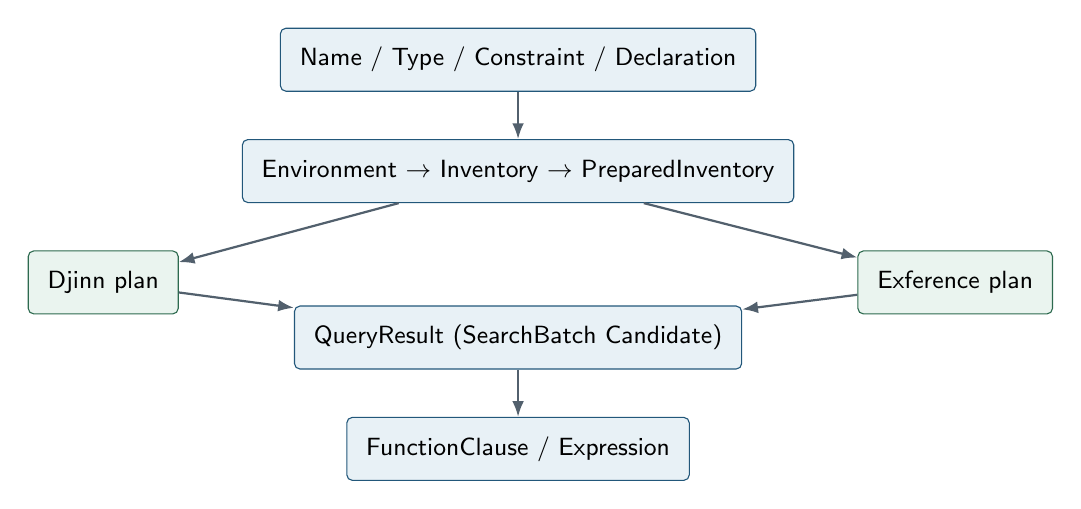
\begin{tikzpicture}[
  node distance=6mm and 8mm,
  every node/.style={font=\small\sffamily},
  box/.style={draw=Accent,rounded corners=2pt,fill=AccentLight,minimum height=8mm,align=center,inner xsep=7pt},
  engine/.style={draw=Green,rounded corners=2pt,fill=GreenLight,minimum height=8mm,align=center,inner xsep=7pt},
  arr/.style={-{Latex[length=2mm]},thick,color=Muted}
]
\node[box] (decl) {Name / Type / Constraint / Declaration};
\node[box,below=of decl] (env) {Environment $\to$ Inventory $\to$ PreparedInventory};
\node[engine,below left=of env] (djinn) {Djinn plan};
\node[engine,below right=of env] (exf) {Exference plan};
\node[box,below=13mm of env] (result) {QueryResult (SearchBatch Candidate)};
\node[box,below=of result] (generated) {FunctionClause / Expression};
\draw[arr] (decl) -- (env);
\draw[arr] (env) -- (djinn);
\draw[arr] (env) -- (exf);
\draw[arr] (djinn) -- (result);
\draw[arr] (exf) -- (result);
\draw[arr] (result) -- (generated);
\end{tikzpicture}
\end{center}

The most important existing properties are these:

\begin{itemize}
  \item \filepath{Query.hs} separates logical evidence from operational progress.
        A candidate discovered before a budget is exhausted remains a valid candidate;
        a truncated empty search is not silently promoted to non-inhabitation.
  \item \filepath{Search.hs} makes truncation reasons explicit and intentionally makes
        no logical claim.
  \item \filepath{Candidate.hs} combines checked generated output, residual type-class
        constraints, and backend-specific details without erasing the latter.
  \item \filepath{Generated.hs} supplies a common scope-aware expression AST, holes,
        alpha equivalence, substitution, bottom-up rewriting, simplification, global
        reference discovery, and expression size.
  \item \filepath{Selection.hs} already contains a monadic, batch-by-batch fold over a
        lazy result trace. This is exactly the primitive needed to run an effectful
        solver filter without forcing the rest of Exference's stream.
  \item \filepath{Declaration.hs} treats neutral declarations as the authority and
        backend caches/ratings as projections. Semantic summaries should follow the
        same pattern.
\end{itemize}

The checked Djinn adapter returns one terminal result batch. The checked Exference
adapter returns a lazy sequence of batches. Both expose shared candidates, but they
retain backend-specific metrics and evidence. This is a strong base for adding a
third, orthogonal concern: semantic contracts.

\subsection{The generated AST is useful but currently too weakly typed}

The shared generated expression contains precisely the constructs needed for symbolic
interpretation:

\begin{lstlisting}[language=HaskellExt,caption={Simplified shape of Djex's shared generated expression}]
data Expression local
  = Local local
  | Global Name
  | Lambda [Pattern local] (Expression local)
  | Apply (Expression local) (Expression local)
  | VisibleTypeApplication (Expression local) VisibleTypeArgument
  | Tuple [Expression local]
  | Hole local
  | Let (Pattern local) (Expression local) (Expression local)
  | Case (Expression local) [(Pattern local, Expression local)]
\end{lstlisting}

However, this is the \emph{checked output} representation after the engines have erased
most private type annotations. A semantic interpreter cannot correctly translate an
arbitrary application, overloaded global, polymorphic instantiation, or case arm from
this tree alone. The integration therefore needs one of two safe boundaries:

\begin{enumerate}
  \item an initial first-order re-elaborator that reconstructs types from the goal and
        the exact inventory, refusing anything ambiguous; or
  \item preferably, a new typed projection emitted at the same point where Djinn's
        proof term and Exference's independently checked expression become the shared
        generated tree.
\end{enumerate}

The second option is the durable design. It preserves the existing public AST and
renderers while attaching a type to every node or stable node path.

\subsection{Exference already has the data needed for deep semantic pruning}

Internally, Exference represents every queued branch as a \code{SearchNode} containing:

\begin{itemize}
  \item a sequence of typed goals, each associated with an expression hole;
  \item the partial typed expression being constructed;
  \item lexical scopes and type substitutions;
  \item provider schemes, deconstructors, constraints, depth, and ranking state.
\end{itemize}

The root starts with a single expression hole. Introduction, tuple, provider,
application, let, and case steps fill one hole and allocate further typed holes. This
is almost exactly a typed sketch state. The obstacle is architectural rather than
representational: the search core is pure. Calling Z3 through
\code{unsafePerformIO} would break cancellation, determinism, exception boundaries,
and referential transparency. The proper refactor is to expose pure branch expansion
and let an outer effectful driver ask a semantic oracle whether a branch is still
feasible.

\subsection{Leant already has the strongest possible final checker}

Leant's \filepath{Leant.Synth.Engine} is deliberately the only module importing Djex.
It translates a Lean goal fragment, invokes Djinn and/or Exference, renders candidate
variants, and returns a bounded ranked stream. In \filepath{Main.hs}, each variant is
then submitted to the active Lean session as a temporary example. A candidate is shown
only if elaboration succeeds, no fatal response occurs, and no \code{sorry} is present.
The generated checker has the shape:

\begin{lstlisting}[language=Lean,caption={Current Leant candidate checking boundary}]
set_option autoImplicit true in
noncomputable example : (goal) := (candidate)
\end{lstlisting}

This is an unusually favorable trust architecture. Z3 can be used aggressively for
search and pruning because a final Leant result need not trust Z3 for type correctness
or for the behavioral theorem. Leant can generate a theorem statement and proof plan,
then ask Lean's kernel to check it.

A necessary representation change is that \code{SynthOutcome} currently returns
rendered strings rather than structured expressions. Semantic filtering should occur
before that erasure, or \code{SynthCandidate} should retain both the Djex expression
and its rendered Lean variants.

\subsection{Z3 capabilities that map directly to this problem}

The pinned Z3 tree exposes all required capabilities through the C API and most
language bindings. The command-line executable also accepts SMT-LIB 2 from standard
input and exposes wall-clock/memory controls, making it a practical zero-FFI MVP.

\begin{longtable}{@{}p{0.25\textwidth}p{0.68\textwidth}@{}}
\toprule
\textbf{Z3 facility} & \textbf{Use in Djex/Leant} \\
\midrule
\endhead
Incremental solver, push/pop & Reuse declaration and contract context across many
candidates and CEGIS iterations. \\
Models and model evaluation & Produce concrete counterexamples, selector assignments,
and synthesized constants. \\
Unsat cores & Explain mutually inconsistent behavioral clauses or infeasible sketch
choices. \\
Optimize & Minimize AST cost, provider cost, case count, literal magnitude, or
contract relaxation lexicographically. \\
Algebraic datatypes & Exact symbolic models for admitted finite inductive data. \\
Sequences and regular expressions & Lists/strings/bytes and regular-language
constraints where sequence semantics is preferable to measures. \\
Arrays and EUF & State maps, finite-memory protocols, bags/count maps, and opaque pure
providers. \\
Bit-vectors & Exact machine arithmetic, masks, packing, bounds, and overflow behavior. \\
Recursive function definitions & Definitional summaries for a controlled structural
fragment. \\
Fixedpoint/PDR (Spacer) & Horn-clause verification, recursive invariants, protocol
reachability, and ranking/invariant synthesis. \\
Proof objects & Optional diagnostics or future independently checked certificates;
not the recommended Leant trust boundary. \\
Interrupt and timeout APIs & Cancellation aligned with Djex/Leant command deadlines. \\
\bottomrule
\end{longtable}

The design should not depend on a SyGuS front end. Ordinary SMT, finite selector
variables, models, blocking clauses, Optimize, and CEGIS are sufficient and give Djex
control over the typed grammar. A repository-wide search of the pinned Z3 revision did
not locate \code{synth-fun} or \code{check-synth} command handling; keeping synthesis
in Djex also avoids coupling the public feature to any future parser-specific support.

\section{The proposed capability: behavioral contracts}

\subsection{A contract is more than a Boolean expression}

A useful contract object must record the quantified program inputs, precondition,
postcondition, semantic domain, admissible abstraction, and proof policy. The following
is representative, not final syntax:

\begin{lstlisting}[language=HaskellExt,caption={Backend-neutral contract vocabulary}]
data Contract ty variable = Contract
  { contractInputs       :: [Binder ty variable]
  , contractPrecondition :: Formula variable
  , contractResult       :: Binder ty variable
  , contractPostcondition :: Formula variable
  , contractDomain       :: SemanticDomain
  , contractMode         :: VerificationMode
  , contractObjectives   :: [Objective]
  }

data SemanticDomain
  = MathematicalTotal
  | FiniteSpineTotal
  | BoundedOperational Bounds

data VerificationMode
  = RequireProof
  | AcceptSolverUnsat
  | AcceptBoundedValidation Bounds
\end{lstlisting}

The checked form should be opaque. Construction validates that every variable is
bound, every operator is sorted, the result type agrees with the type query, all
referenced measures are available, and the selected semantic domain admits every
provider the search may use.

\subsection{Contracts should be elaborated in the source language}

Neither Djex nor Z3 should parse arbitrary Lean terms. Likewise, the solver layer
should not guess the meaning of arbitrary Haskell source text.

\begin{itemize}
  \item A Haskell/Djex frontend parses a compact contract DSL and resolves names through
        the same exact inventory used by synthesis.
  \item Leant asks Lean to elaborate both the type and the contract. A Lean metaprogram
        serializes the elaborated semantic fragment into a canonical S-expression,
        just as the current goal serializer already does for types.
  \item The neutral Djex contract layer receives only checked names, sorts, measures,
        and formulas. No source-language name resolution leaks into Z3 encoding.
\end{itemize}

This arrangement avoids a class of subtle bugs involving namespace aliases, implicit
arguments, overloaded notation, coercions, reducibility, and universes.

\subsection{The central verification query is existential}

Suppose a candidate denotes a total function $f$ and the contract is

\[
  \forall x.\; P(x) \Rightarrow Q(x, f(x)).
\]

Do not ask Z3 to prove this universal formula directly. Ask it for a counterexample:

\[
  \exists x.\; P(x) \land \neg Q(x, f(x)).
\]

The program inputs are declared as free constants. Then:

\begin{itemize}
  \item \code{sat} gives a concrete counterexample model;
  \item \code{unsat} establishes the contract relative to the exact encoding and
        asserted semantic summaries;
  \item \code{unknown} remains unknown, with Z3's reason retained.
\end{itemize}

This quantifier-free or lightly quantified shape is usually much more robust than a
universal theorem. It also fits CEGIS naturally.

\subsection{Semantic summaries are a checked inventory, not annotations sprinkled on terms}

Add a separate \code{SemanticInventory} keyed by Djex's exact structural \code{Name}.
Each entry states what a provider means in one or more abstraction domains:

\begin{lstlisting}[language=HaskellExt,caption={Provider summary sketch}]
data ProviderSummary = ProviderSummary
  { summaryProvider :: Name
  , summaryScheme   :: CheckedSemanticScheme
  , summaryClauses  :: [SummaryClause]
  , summaryTrust    :: SummaryTrust
  , summaryOrigin   :: SummaryOrigin
  }

data SummaryTrust
  = DerivedFromDatatypeDeclaration
  | LeanKernelChecked TheoremName
  | BuiltinAxiom SemanticModelVersion
  | UserAssumed SourceLocation
  | ObservedOnly Bounds
\end{lstlisting}

Constructor summaries can be derived mechanically from a checked
\code{DataTypeDeclaration}. For example, a list constructor has length summary
$\operatorname{len}(\texttt{Cons}\;x\;xs)=1+\operatorname{len}(xs)$. A Lean provider
summary should normally be admitted only when a theorem with the expected shape is
kernel-checked. Haskell summaries may initially be builtin or explicitly assumed; the
result must expose that trust.

Do not overload \code{Declaration}'s opaque annotation field with semantic meaning.
Annotations are source metadata; semantic summaries have versioning, proof origin,
and domain applicability that deserve their own checked index.

\subsection{Use products of abstractions}

No single encoding is best for all contracts. A candidate may be interpreted in a
product of independently selected domains:

\begin{itemize}
  \item \textbf{Measure domain:} length, size, height, constructor counts, numeric bounds.
  \item \textbf{Sequence domain:} element order and concatenation.
  \item \textbf{Bag/provenance domain:} multiplicities or element-origin tokens.
  \item \textbf{Scalar domain:} integers, rationals, bit-vectors, Booleans.
  \item \textbf{Shape domain:} datatype constructor/tag information.
  \item \textbf{State domain:} arrays/maps and protocol state.
  \item \textbf{Opaque domain:} uninterpreted functions with congruence only.
\end{itemize}

The contract compiler requests only the domains it needs, and every provider must have
a compatible summary in each requested domain. This keeps a length-preservation query
in quantifier-free linear integer arithmetic instead of unnecessarily encoding entire
lists.

\section{Architecture}

\subsection{Dependency direction}

The clean architecture is a four-layer stack:

\begin{center}
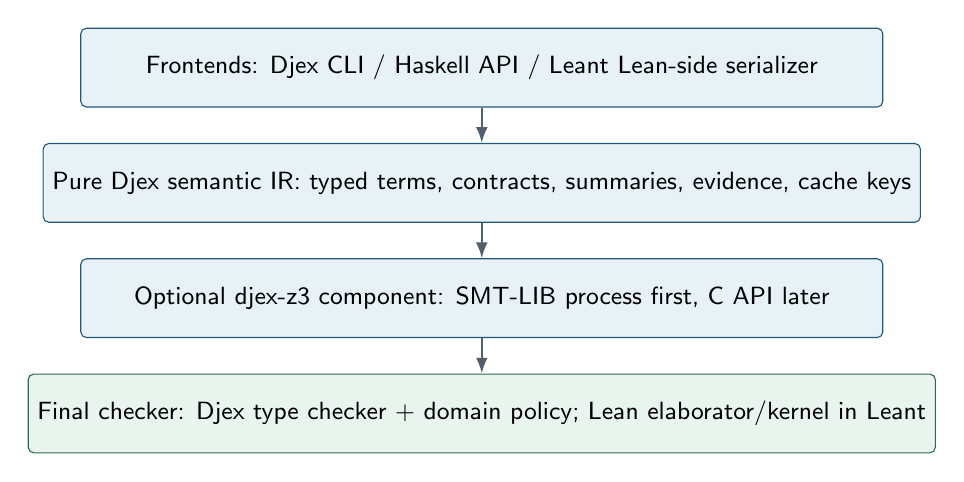
\begin{tikzpicture}[
  node distance=4.5mm,
  every node/.style={font=\small\sffamily,align=center},
  layer/.style={draw=Accent,fill=AccentLight,rounded corners=2pt,minimum width=0.84\textwidth,minimum height=10mm},
  trusted/.style={draw=Green,fill=GreenLight,rounded corners=2pt,minimum width=0.84\textwidth,minimum height=10mm},
  arr/.style={-{Latex[length=2mm]},thick,color=Muted}
]
\node[layer] (front) {Frontends: Djex CLI / Haskell API / Leant Lean-side serializer};
\node[layer,below=of front] (neutral) {Pure Djex semantic IR: typed terms, contracts, summaries, evidence, cache keys};
\node[layer,below=of neutral] (solver) {Optional djex-z3 component: SMT-LIB process first, C API later};
\node[trusted,below=of solver] (check) {Final checker: Djex type checker + domain policy; Lean elaborator/kernel in Leant};
\draw[arr] (front) -- (neutral);
\draw[arr] (neutral) -- (solver);
\draw[arr] (solver) -- (check);
\end{tikzpicture}
\end{center}

The neutral semantic IR belongs close to Djex's existing synthesis foundation and must
remain pure. Solver process management and FFI handles belong in a separate optional
component. This preserves lightweight use of Djex when no Z3 executable or library is
available and prevents solver state from contaminating pure search code.

\subsection{New neutral modules}

A plausible module layout is:

\begin{lstlisting}[language=HaskellExt]
Language.Haskell.Synthesis.TypedGenerated
Language.Haskell.Synthesis.Semantic.Sort
Language.Haskell.Synthesis.Semantic.Term
Language.Haskell.Synthesis.Semantic.Formula
Language.Haskell.Synthesis.Semantic.Contract
Language.Haskell.Synthesis.Semantic.Measure
Language.Haskell.Synthesis.Semantic.Summary
Language.Haskell.Synthesis.Semantic.Inventory
Language.Haskell.Synthesis.Semantic.Elaborate
Language.Haskell.Synthesis.Semantic.Symbolic
Language.Haskell.Synthesis.Semantic.Evidence
Language.Haskell.Synthesis.Semantic.CacheKey
\end{lstlisting}

The Z3-specific package or Cabal component can then provide:

\begin{lstlisting}[language=HaskellExt]
Language.Haskell.Synthesis.Z3.Session
Language.Haskell.Synthesis.Z3.SExpr
Language.Haskell.Synthesis.Z3.SMTLib
Language.Haskell.Synthesis.Z3.Encode
Language.Haskell.Synthesis.Z3.Model
Language.Haskell.Synthesis.Z3.Optimize
Language.Haskell.Synthesis.Z3.Fixedpoint
Language.Haskell.Synthesis.Z3.Verify
\end{lstlisting}

Leant-specific code should stay behind its present narrow engine boundary:

\begin{lstlisting}[language=HaskellExt]
Leant.Synth.Contract
Leant.Synth.Semantic
Leant.Synth.ProofPlan
Leant.Z3
\end{lstlisting}

\subsection{Retaining typed generated terms}

The recommended representation is a checked shared tree with a type at every node,
plus a projection to today's \code{Expression}:

\begin{lstlisting}[language=HaskellExt,caption={One possible typed output boundary}]
data TypedExpression ty local = TypedExpression
  { typedExpressionType :: !ty
  , typedExpressionNode :: TypedNode ty local
  }

data TypedNode ty local
  = TLocal local
  | TGlobal Name [VisibleTypeArgument]
  | TLambda [(Pattern local, ty)] (TypedExpression ty local)
  | TApply (TypedExpression ty local) (TypedExpression ty local)
  | TTuple [TypedExpression ty local]
  | THole HoleId ty
  | TLet (Pattern local) (TypedExpression ty local)
         (TypedExpression ty local)
  | TCase (TypedExpression ty local)
          [(TypedPattern ty local, TypedExpression ty local)]

eraseTypes :: TypedExpression ty local -> Expression local
\end{lstlisting}

An alternative, less invasive form is an \code{ElaboratedCandidate} containing the
existing expression and a total map from stable node paths to types. The tree form is
harder to desynchronize and is better for sketch synthesis; the side-table form may be
useful as a compatibility bridge.

Typed output should be produced before backend erasure:

\begin{itemize}
  \item in Djinn, while projecting the proof term to generated syntax;
  \item in Exference, from the independently checked internal expression after type
        substitutions and constraint resolution, before projecting to shared syntax.
\end{itemize}

The existing candidate and renderer APIs remain source-compatible. New constrained
APIs can request typed output explicitly.

\subsection{Do not overload existing evidence}

Use an orthogonal wrapper:

\begin{lstlisting}[language=HaskellExt,caption={Separate type-search and semantic evidence}]
data SemanticVerdict
  = ContractProved ProofBasis
  | ContractRefuted Counterexample
  | ContractValidatedWithin Bounds ValidationSummary
  | ContractUnknown UnknownReason

data ProofBasis
  = LeanKernelChecked TheoremName
  | Z3Unsat SolverFingerprint EncodingFingerprint
  | CertificateChecked CertificateFingerprint
  | ExactNormalization SemanticModelVersion

data ConstrainedCandidate candidate = ConstrainedCandidate
  { constrainedCandidate :: candidate
  , constrainedVerdict   :: SemanticVerdict
  , constrainedCost      :: SemanticCost
  }

data ConstrainedResult metadata candidate = ConstrainedResult
  { typeSearchResult :: QueryResult metadata candidate
  , semanticResults  :: [ConstrainedCandidate candidate]
  , semanticProgress :: SolverProgress
  }
\end{lstlisting}

This prevents several invalid inferences. In particular:

\begin{itemize}
  \item Djinn can prove that a type is inhabited while every inspected inhabitant fails
        a behavioral contract.
  \item Exference can be truncated after every inspected candidate fails; this is not
        proof that no satisfying term exists.
  \item Z3 can return \code{unsat} for a candidate under assumed provider summaries;
        this is not the same as a Lean-kernel theorem.
  \item A finite grammar can be exhausted semantically even though the unrestricted
        type has other inhabitants outside the grammar.
\end{itemize}

\subsection{Completeness and trust are a vector}

Every constrained synthesis answer should carry at least these independent dimensions:

\begin{longtable}{@{}p{0.28\textwidth}p{0.63\textwidth}@{}}
\toprule
\textbf{Dimension} & \textbf{Representative values} \\
\midrule
\endhead
Type-search status & complete, candidate-bounded, step-bounded, queue-pruned,
identifier-space exhausted. \\
Grammar status & unrestricted calculus, exact finite grammar, size-bounded grammar,
provider-bounded grammar. \\
Semantic translation & exact for admitted fragment, abstraction-sound but incomplete,
bounded execution, unsupported. \\
Provider trust & derived constructor, Lean theorem, builtin axiom, user assumption,
observed sample. \\
Solver status & sat with model, unsat, unknown with reason, timeout, interrupted,
protocol failure. \\
Final checking & Lean kernel theorem, source-language typecheck only, independently
checked certificate, solver-only, testing-only. \\
\bottomrule
\end{longtable}

A concise UI can summarize this vector, but the structured API must not collapse it.


\section{Algorithms}

\subsection{Mode 1: streaming semantic post-filtering}

This mode can be implemented without changing either search calculus. It is the right
first milestone because it establishes contract elaboration, semantic summaries, Z3
transport, evidence, counterexamples, caching, cancellation, and UI semantics before
any search-internal changes.

For each complete candidate:

\begin{enumerate}
  \item obtain or reconstruct its typed generated expression;
  \item select the semantic domains required by the contract;
  \item symbolically interpret the expression using exact constructor semantics and
        checked provider summaries;
  \item assert the negated postcondition under the precondition;
  \item ask Z3 for satisfiability;
  \item retain \code{unsat} candidates, report models for \code{sat}, and preserve
        \code{unknown} according to caller policy.
\end{enumerate}

Pseudocode:

\begin{lstlisting}[language=HaskellExt,caption={Streaming post-filtering over existing result batches}]
filterConstrained
  :: SolverSession
  -> CheckedContract
  -> SemanticInventory
  -> [QueryResult metadata candidate]
  -> IO (Maybe Progress, ConstrainedAccumulator candidate)
filterConstrained solver contract inventory =
  foldAllQueryResultsM admissible inspect emptyAccumulator
 where
  admissible = candidateHasNoUnsupportedResiduals

  inspect acc candidate = do
    typed <- requireTypedCandidate candidate
    case symbolicInterpret inventory contract typed of
      Left unsupported ->
        pure (recordUnknown candidate unsupported acc)
      Right interpretation -> do
        verdict <- verifyCounterexampleQuery solver contract interpretation
        pure (record candidate verdict acc)
\end{lstlisting}

The use of Djex's existing \code{foldAllQueryResultsM} is important. It preserves
Exference's laziness, permits short-circuiting after the requested number of satisfying
candidates, and does not retain the root of a large result trace. Djinn's single
terminal batch passes through the same API.

A useful result-selection policy is not merely ``keep all unsat candidates''. It should
support:

\begin{itemize}
  \item first proof-grade candidate;
  \item best $k$ candidates under a combined syntactic/semantic cost;
  \item first candidate in each semantic equivalence class;
  \item proof-grade candidates preferred, bounded candidates as fallback;
  \item stop after $n$ solver checks without improvement.
\end{itemize}

\subsection{Mode 2: counterexample-guided typed sketch synthesis}

Post-filtering wastes work when a behavioral contract is selective. The next step is
to let Z3 choose among a finite, type-correct set of construction alternatives.
Djex remains responsible for the typed grammar; Z3 never invents an untyped program.

A typed hole $h_i : \tau_i$ receives alternatives
$e_{i,0},\ldots,e_{i,k_i-1}$ generated from the lexical context, constructors, and
provider inventory. Introduce an integer or bit-vector selector $s_i$ with
$0 \leq s_i < k_i$. The symbolic value of the hole is:

\[
  \llbracket h_i \rrbracket =
  \operatorname{ite}(s_i=0,\llbracket e_{i,0}\rrbracket,
    \operatorname{ite}(s_i=1,\llbracket e_{i,1}\rrbracket,\ldots)).
\]

The first implementation should use an acyclic grammar and a strict AST-size bound.
Recursive calls can be admitted later under structural decrease and CHC verification.
The synthesis loop is CEGIS:

\begin{lstlisting}[language=HaskellExt,caption={Typed CEGIS loop}]
cegis :: Sketch -> CheckedContract -> IO SynthesisOutcome
cegis sketch contract = loop initialExamples
 where
  loop examples = do
    model <- solveSelectors sketch contract examples
    case model of
      Unsat -> pure NoProgramInGrammar
      Unknown why -> pure (SynthesisUnknown why)
      Sat assignment -> do
        let candidate = decodeSketch sketch assignment
        counterexample <- verifyCandidate contract candidate
        case counterexample of
          Unsat -> pure (Found candidate)
          Sat input -> loop (input : examples)
          Unknown why -> pure (CandidateUnknown candidate why)
\end{lstlisting}

The synthesis query constrains the candidate on a growing finite example set. The
verification query asks existentially for a fresh counterexample over the full admitted
symbolic domain. Blocking only the complete selector vector is correct but slow;
learned clauses should instead block the smallest responsible subassignment when
possible.

\subsubsection{Why this is preferable to generic syntax synthesis in Z3}

\begin{itemize}
  \item The grammar is produced from Djex's exact type environment, including local
        scopes, constructors, higher-rank boundaries, visible type applications, and
        provider instantiations.
  \item Every decoded model denotes a well-scoped, type-correct candidate by
        construction.
  \item Djex can retain its own term-size and provider-rating heuristics.
  \item The encoding can exploit domain-specific summaries without exposing Haskell or
        Lean syntax to Z3.
  \item Grammar exhaustion has a precise, reportable meaning.
\end{itemize}

\subsection{Mode 3: semantic pruning of Exference search nodes}

Exference is particularly suitable for incremental semantic pruning because each
search node already contains a partial expression and a set of typed holes. The
semantic oracle should compute a \emph{necessary} condition for some completion of the
node to satisfy the contract. If that condition is unsatisfiable, the branch is safe to
prune. A satisfiable result is only feasibility evidence, not proof that a completion
exists.

A clean refactor is:

\begin{lstlisting}[language=HaskellExt,caption={Effectful driver around a pure search step}]
data SearchExpansion node candidate
  = Solved candidate
  | Expanded [node]
  | DeadEnd

stepExference :: SearchNode -> SearchExpansion SearchNode Candidate

class Monad m => SemanticOracle m node where
  classifyNode :: CheckedContract -> node -> m BranchVerdict

data BranchVerdict
  = DefinitelyInfeasible UnsatExplanation
  | PossiblyFeasible SemanticLowerBound
  | OracleUnknown UnknownReason
\end{lstlisting}

The outer driver pops a node, calls \code{stepExference}, and batches semantic queries
for children. Only \code{DefinitelyInfeasible} removes a child. The lower bound may be
added to Exference's priority to rank branches that are semantically closer to the
contract.

The abstraction for a hole must be permissive. For example, if a hole of list type can
be filled only from a finite grammar whose possible length transforms are
$\{n,0,n+1\}$, then the branch can use the disjunction. If no finite grammar is fixed,
the hole's length must be an unconstrained nonnegative integer; otherwise pruning could
be unsound.

\subsubsection{Oracle call control}

A solver call per branch would overwhelm small searches. Use:

\begin{itemize}
  \item checks only after semantic milestones (provider choice, constructor choice,
        branch predicate, recursive call), not every administrative transition;
  \item batched sibling checks with assumptions and unsat cores;
  \item a cheap abstract interpreter before Z3;
  \item memoization by alpha-normalized partial term, normalized type substitution,
        contract, and semantic inventory fingerprint;
  \item adaptive checking: increase solver frequency only after the queue exceeds a
        threshold or the contract rejects a high fraction of completed candidates.
\end{itemize}

\subsection{Optimize-based ranking}

Z3 Optimize should not replace Djex's mature search ranking at first. It is most useful
inside a finite sketch or after candidate generation. A lexicographic objective can be:

\[
  (\text{proof grade},\;\text{AST size},\;\text{provider cost},\;
   \text{case count},\;\text{literal magnitude},\;\text{semantic distance}).
\]

Hard constraints establish typing and behavior. Soft constraints prefer the original
input, avoid unsafe/assumed summaries, preserve all arguments, or use highly rated
providers. The model must be decoded and rechecked by the ordinary solver because
optimization plus quantified or recursive constraints may return \code{unknown} or
non-obvious bounds.

\subsection{Fixedpoint/PDR for recursive programs}

Recursive synthesis should not begin by expanding recursive functions into bounded
traces and calling that proof. Z3's Fixedpoint API accepts universal Horn clauses and
supports PDR-style queries with background assertions. This maps naturally to:

\begin{itemize}
  \item relational semantics of a recursive function;
  \item a safety predicate representing the behavioral law;
  \item unknown inductive invariants from a template family;
  \item ranking functions or structural decrease conditions.
\end{itemize}

For a recursive list transformer, define a relation
$F(xs,ys)$, constructor rules for the program, and a bad relation
$\operatorname{Bad}(xs,ys)$ when the contract fails. Query reachability of
\code{Bad}. Fixedpoint \code{false} establishes safety in the CHC encoding; the answer
or cover can help reconstruct an invariant. In Leant, that invariant becomes a hint for
an induction proof, not a trusted theorem by itself.

\section{Worked example: a polymorphic list transformer preserving length}
\label{sec:length-example}

\subsection{Semantic statement}

The surface request is:

\begin{lstlisting}[language=HaskellExt]
f :: [a] -> [a]
-- Contract: for every admitted xs,
--           length (f xs) = length xs
\end{lstlisting}

For Haskell, the first proof-grade semantic mode should define ``admitted'' as:

\begin{itemize}
  \item \code{xs} has a finite, total spine;
  \item element payloads need not be evaluated by a length-only contract;
  \item the candidate belongs to the total structural fragment and cannot use bottom,
        exceptions, \code{seq}, unsafe casts, effects, or unrestricted recursion;
  \item every referenced provider has a compatible total summary.
\end{itemize}

Let $n=\operatorname{len}(xs)$ with $n\geq0$. A length summary maps the candidate to an
integer term $L_f(n)$. Verification asks whether

\[
  n\geq0 \land L_f(n)\neq n
\]

is satisfiable.

\subsection{What Z3 says about common candidates}

\begin{longtable}{@{}p{0.25\textwidth}p{0.28\textwidth}p{0.37\textwidth}@{}}
\toprule
\textbf{Candidate shape} & \textbf{Length summary} & \textbf{Counterexample query} \\
\midrule
\endhead
\code{\textbackslash xs -> xs} & $n$ & Unsatisfiable. \\
\code{\textbackslash \_ -> []} & $0$ & $n=1$ is a model. \\
\code{tail} with totalized empty case & $\operatorname{ite}(n=0,0,n-1)$ & $n=1$ is a model. \\
\code{\textbackslash xs -> xs ++ xs} & $2n$ & $n=1$ is a model. \\
\code{reverse} & $n$ under a checked summary & Unsatisfiable. \\
\code{drop k} & $\max(n-k,0)$ & For fixed $k>0$, $n=1$ is usually a model; only $k=0$ works universally. \\
\code{take k} & $\min(k,n)$ & $n=k+1$ is a model for finite $k$. \\
\code{\textbackslash (x:xs) -> xs ++ [x]} with empty case & $n$ & Unsatisfiable in the length domain. \\
\bottomrule
\end{longtable}

The last row is deliberately important: length preservation is not identity. The
contract admits reverse, rotations, arbitrary permutations, and even some programs
that drop and duplicate elements in a balanced way. This is a feature, not a bug. A
user who wants a permutation should add bag equality; a user who wants identity should
state extensional equality.

\subsection{Minimal SMT-LIB verification}

For a candidate whose summary is $2n$:

\begin{lstlisting}[language=SMTLIB,caption={Counterexample query for duplicating the list}]
(set-logic QF_LIA)
(set-option :produce-models true)
(declare-const n Int)
(assert (>= n 0))
(define-fun outLen () Int (* 2 n))
(assert (not (= outLen n)))
(check-sat)
(get-value (n outLen))
\end{lstlisting}

A conforming response includes a model such as $n=1$, $\texttt{outLen}=2$. For the
identity summary, the final assertion simplifies to $n\neq n$ and the result is
\code{unsat}.

The actual session should not emit a new declaration context for every candidate. It
should push a candidate scope, assert the candidate-specific definition and bad
condition, check, obtain model/core if applicable, then pop.

\subsection{A first typed grammar}

For a deliberately small grammar over \code{xs :: [a]}:

\[
\begin{aligned}
E_{[a]} ::=\;& xs \mid [] \mid \operatorname{reverse}(E_{[a]})
              \mid E_{[a]} \mathbin{++} E_{[a]} \\
            &\mid \operatorname{tail0}(E_{[a]})
              \mid \operatorname{take}(E_{\mathbb{N}},E_{[a]})
              \mid \operatorname{drop}(E_{\mathbb{N}},E_{[a]}) \\
E_{\mathbb{N}} ::=\;& 0 \mid 1 \mid n \mid E_{\mathbb{N}}+E_{\mathbb{N}}.
\end{aligned}
\]

Every constructor has a length transfer function. Z3 can select a term of bounded
size, constrain its transfer function to equal $n$ on accumulated examples, and then
verify the decoded term for all $n\geq0$. Optimize minimizes size and provider cost.

A first synthesis result is likely identity because it has minimum size. Add a novelty
constraint to request a nontrivial solution:

\[
  \exists xs.\; f(xs)\neq xs,
\]

or ban the direct variable alternative. The next minimal candidate may be reverse or a
single rotation, depending on the inventory and cost model.

\subsection{Adding bag preservation}

Length plus bag equality gives a permutation law:

\[
  \operatorname{len}(f(xs))=\operatorname{len}(xs)
  \quad\land\quad
  \operatorname{bag}(f(xs))=\operatorname{bag}(xs).
\]

For a bounded element universe, a bag can be an array from element tokens to integer
counts. For an unbounded parametric universe, use provenance tokens introduced for
input positions and constrain constructors/providers by their token transfer. In the
pure parametric structural fragment, this is closely related to a free theorem, but the
implementation should not silently assume parametricity when providers may use
\code{seq}, type reflection, unsafe features, or effects.

A sequence-domain encoding can prove order-sensitive laws directly, but measure plus
provenance domains are often much cheaper and provide better counterexamples.

\subsection{Leant form of the same query}

A possible surface syntax is:

\begin{lstlisting}[language=Lean]
:synth (f : List alpha -> List alpha)
  where forall xs, (f xs).length = xs.length
\end{lstlisting}

The displayed ASCII spelling is only illustrative; the real parser should let Lean
elaborate ordinary Lean syntax, including implicit parameters and notation. A successful
proof-grade result can be presented as:

\begin{lstlisting}[language=Lean]
it1 : List alpha -> List alpha := fun xs => xs
it1_spec : forall xs, (it1 xs).length = xs.length := by
  intro xs
  rfl
\end{lstlisting}

For a rotation or recursive transformer, the generated proof plan may use induction,
\code{simp}, and \code{omega}. The theorem, not Z3's \code{unsat}, is the final trusted
artifact.

\section{Djex integration in detail}

\subsection{Public API shape}

The constrained API should be additive. Existing calls retain their exact semantics.
One possible high-level interface is:

\begin{lstlisting}[language=HaskellExt,caption={Additive constrained-query API}]
data ConstrainedRequest ty options = ConstrainedRequest
  { constrainedTypeRequest :: QueryRequest ty options
  , constrainedContract    :: CheckedContract
  , constrainedPolicy      :: ConstrainedPolicy
  }

data ConstrainedPolicy = ConstrainedPolicy
  { semanticUnknownPolicy :: UnknownPolicy
  , maximumSolverChecks   :: Maybe Natural
  , requiredProofGrade    :: ProofGrade
  , semanticSelection     :: SemanticSelection
  }

runDjinnConstrained
  :: Z3Session
  -> SemanticInventory
  -> DjinnSession
  -> ConstrainedRequest DjinnType QueryOptions
  -> IO (Either Diagnostic DjinnConstrainedResult)

runExferenceConstrained
  :: Z3Session
  -> SemanticInventory
  -> ExferenceSession
  -> ConstrainedRequest ExferenceType ExferenceOptions
  -> IO (Either Diagnostic [ExferenceConstrainedResult])
\end{lstlisting}

An even cleaner API separates search from verification so applications can reuse a
candidate stream or substitute another solver backend:

\begin{lstlisting}[language=HaskellExt]
verifyCandidate
  :: MonadSemanticSolver m
  => CheckedSemanticContext
  -> TypedCandidate
  -> m SemanticVerdict

foldConstrainedResultsM
  :: Monad m
  => (candidate -> m SemanticVerdict)
  -> ConstrainedFoldPolicy
  -> [QueryResult metadata candidate]
  -> m (ConstrainedSelection candidate)
\end{lstlisting}

The Z3 package then instantiates \code{MonadSemanticSolver}; tests can use a mock or a
small exhaustive evaluator.

\subsection{Session construction and inventory fingerprints}

A checked semantic session should seal:

\begin{itemize}
  \item the exact neutral declaration inventory;
  \item normalized provider summaries and their proof origins;
  \item datatype-derived measures;
  \item semantic model version;
  \item solver capabilities/version;
  \item namespace mapping from Djex names to collision-free SMT symbols.
\end{itemize}

Like current Djinn/Exference sessions, this moves fallible validation out of the lazy
query result. A malformed summary, unsupported recursive measure, or conflicting name
must fail before \code{Right} exposes a result stream.

A fingerprint should cover structural content, not rendered spelling. It belongs in
cache keys and result evidence so a result cannot be replayed after a provider theorem
or semantic axiom changes.

\subsection{Source-level contract syntax for Djex}

A minimal CLI syntax might be:

\begin{lstlisting}[language=HaskellExt]
lengthPreserving ? f :: [a] -> [a]
  where forall xs. length (f xs) == length xs
\end{lstlisting}

or a command-oriented form:

\begin{lstlisting}[language=HaskellExt]
:contract f :: [a] -> [a]
  ensures length result == length arg0
:solve f
\end{lstlisting}

The parser should lower names such as \code{length} to checked semantic measure IDs,
not ordinary executable globals. Start with a compact first-order grammar:

\begin{itemize}
  \item Boolean connectives and equality/order;
  \item integer and bit-vector arithmetic;
  \item named measures on arguments/result;
  \item constructor/tag tests;
  \item array/sequence operations admitted by selected domains;
  \item explicit quantification over finite auxiliary domains only.
\end{itemize}

Do not start by embedding arbitrary Haskell expressions in contracts. That would
immediately inherit bottoms, type classes, laziness, desugaring, and module-resolution
complexity.

\subsection{Residual constraints and dictionary semantics}

Djex candidates may retain type-class obligations. A constrained query must decide
whether they are:

\begin{itemize}
  \item fully resolved before semantic interpretation;
  \item admitted as exact provider assignments with semantic summaries; or
  \item rejected/marked unsupported.
\end{itemize}

Treating a residual class constraint as an uninterpreted Boolean assumption is usually
unsound for behavioral laws because the selected dictionary controls method behavior.
The semantic inventory must attach summaries to the exact resolved provider or to a
class law that is valid for every admitted instance.

\subsection{Preserving laziness and cancellation}

The constrained layer is effectful, but the candidate list may remain lazy. Use a
producer/consumer discipline:

\begin{itemize}
  \item force only enough of the next candidate to type/semantically elaborate it;
  \item check candidates under a bounded worker pool, preserving deterministic result
        order unless the caller explicitly selects fastest-first mode;
  \item propagate asynchronous exceptions; do not convert them to semantic unknowns;
  \item on cancellation, send \code{Z3\_interrupt} for FFI sessions or terminate and
        restart a subprocess session if protocol synchronization cannot be guaranteed;
  \item retain the last inspected Djex progress and a separate solver progress.
\end{itemize}

\subsection{Semantic deduplication before rendering}

Djex already supports alpha equivalence and structural simplification. Add an optional
semantic equivalence check:

\[
  \exists x.\; \llbracket f(x)\rrbracket \neq \llbracket g(x)\rrbracket.
\]

If unsatisfiable in the requested observation domain, put $f$ and $g$ in the same
semantic class and present the syntactically smallest or best-rated representative.
This can dramatically reduce Exference's repeated derivations and near-duplicates.
The UI must say ``equivalent under length/bag observations'', not ``extensionally equal'',
unless the encoding is exact for full values.

\section{Leant integration in detail}

\subsection{Elaborate the contract in Lean}

Leant's existing serializer is the model. Add a Lean metaprogram that receives the
elaborated function type and contract, then emits a canonical semantic fragment. It
should recognize an intentionally bounded vocabulary:

\begin{itemize}
  \item propositions, equality, order, connectives, and quantifiers;
  \item \code{Nat}, \code{Int}, and fixed-width bit-vector operations;
  \item list/array/string measures and selected operations;
  \item constructors and non-dependent finite inductives;
  \item theorem-backed provider summaries registered by an attribute.
\end{itemize}

Anything else is returned as a structured refusal or opaque atom according to policy.
As with the type serializer, pretty-printed source text is for diagnostics only; exact
Lean names and elaborated structure are the authority.

A possible theorem-summary declaration is:

\begin{lstlisting}[language=Lean]
@[leant_synth_summary]
theorem List.reverse_length (xs : List alpha) :
    (List.reverse xs).length = xs.length := by
  simp
\end{lstlisting}

The attribute handler checks that the theorem matches a supported summary schema and
serializes its exact constant name, quantified variables, preconditions, and equation.
A stale or ill-shaped declaration fails summary registration rather than silently
becoming an assumption.

\subsection{Retain structured candidates in the engine}

Replace or supplement:

\begin{lstlisting}[language=HaskellExt]
SynthCandidates [[String]] [String]
\end{lstlisting}

with:

\begin{lstlisting}[language=HaskellExt]
data SynthCandidate = SynthCandidate
  { synthExpression  :: Expression String
  , synthTypedView   :: Maybe LeantTypedCandidate
  , synthVariants    :: [String]
  , synthOrigin      :: SynthEngine
  , synthMetrics     :: CandidateMetrics
  }

data SynthOutcome
  = SynthCandidates [SynthCandidate] [String]
  | SynthRefuted RefutationStrength
  | SynthNoTerm [String]
\end{lstlisting}

This keeps today's rendering variants and scheduling logic while allowing semantic
verification before or after rendering. The engine remains swappable because the
structured candidate is still Djex-neutral rather than an Exference node.

\subsection{Verification pipeline}

For a proof-grade constrained query, process each candidate in this order:

\begin{enumerate}
  \item \textbf{Lean type check.} Submit today's temporary example to the actual user
        environment. This catches renderer, namespace, implicit-argument, and universe
        errors.
  \item \textbf{Z3 semantic check.} Encode the exact admitted contract fragment and ask
        for a counterexample. Reject \code{sat}; retain the model for explanation.
  \item \textbf{Proof-plan generation.} Translate the symbolic derivation, candidate
        shape, and solver facts into a small Lean tactic plan.
  \item \textbf{Lean theorem check.} Submit a temporary theorem binding the candidate
        and proving the contract. Accept proof-grade status only if Lean reports no
        errors or sorries.
  \item \textbf{Binding.} Bind both candidate and theorem in the REPL's usual
        \code{it}-style order.
\end{enumerate}

A generic generated checker is:

\begin{lstlisting}[language=Lean,caption={Final Leant behavioral checker shape}]
set_option autoImplicit true in
noncomputable example :
  let f : TargetType := candidate
  Contract f := by
    proof_plan
\end{lstlisting}

For simple definitional laws the plan is \code{rfl} or \code{simp}. For Presburger
residuals it can be \code{simp [candidate, summaries] <;> omega}. For structural
recursion it can be induction followed by simplification and arithmetic.

\subsection{Proof-plan reconstruction tiers}

The proof generator should be deliberately modest and compositional:

\begin{enumerate}
  \item definitional reduction / \code{rfl};
  \item rewriting by exact registered summary theorems;
  \item \code{simp} normalization;
  \item \code{omega} for natural/integer linear arithmetic;
  \item constructor congruence and extensionality;
  \item induction on one structurally decreasing argument;
  \item explicit case splits corresponding to candidate cases;
  \item only later, imported proof certificates or richer tactic search.
\end{enumerate}

Z3 models and unsat cores help choose splits and lemmas. They do not have to be
translated into a general proof object. This avoids making Leant depend on the full
stability and semantics of Z3's internal proof AST.

\subsection{User-facing commands}

A coherent command family could be:

\begin{lstlisting}[language=Lean]
:synth (f : List alpha -> List alpha)
  where forall xs, (f xs).length = xs.length

:set synth-contract-proof kernel|solver|bounded
:set synth-semantic-domain length,bag
:set synth-z3-timeout 1500
:set synth-counterexamples on
:set synth-semantic-dedupe on
\end{lstlisting}

Output should distinguish results explicitly:

\begin{lstlisting}
1. fun xs => xs
   contract: proved by Lean kernel (rfl)

rejected: fun _ => []
   counterexample: input length = 1, output length = 0

search note: Exference queue pruned 247 nodes
solver note: 8 candidates checked, 5 counterexamples, 2 semantic duplicates
\end{lstlisting}

When the type search itself yields a Djinn refutation, Leant can still report it under
its current safety rules. When a finite semantic grammar is exhausted, say
``no satisfying program in grammar of size at most $k$ using these providers'', never
``no term exists''.

\subsection{Proof-producing synthesis as a first-class feature}

The strongest Leant feature is not merely filtering terms. It is synthesizing a pair:

\[
  (f,\;p) \quad\text{where}\quad p : \forall x,\;P(x)\to Q(x,f(x)).
\]

The REPL can bind:

\begin{lstlisting}[language=Lean]
it1      : TargetType := ...
it1_spec : Contract it1 := by ...
\end{lstlisting}

This makes synthesized results reusable in later proofs, exportable to source, and
independent of the solver after kernel checking. It also creates a natural feedback
loop: newly proved summaries can be registered as providers for subsequent synthesis.


\section{High-value features unlocked by the same integration}

Behavioral term synthesis is the core, but several features become available almost
for free once typed candidates, semantic summaries, and a persistent solver session
exist.

\subsection{Minimal counterexamples for every rejected candidate}

A type-only synthesizer can say that a term has the requested type. A semantic
synthesizer can say exactly why it is wrong. Z3 models should be decoded back through
the semantic domain:

\begin{itemize}
  \item list length, constructor skeleton, and selected provenance positions;
  \item concrete integers/bit-vectors and overflow flags;
  \item protocol state and event sequence;
  \item finite map entries or array indices on which outputs differ.
\end{itemize}

Then minimize the model. For arithmetic, optimize lexicographically by input size and
absolute values. For ADTs, minimize constructor count. For sequences, minimize length
and then lexicographic token values. A small counterexample is often more valuable to a
user than a rejected/accepted bit.

Counterexamples can also seed regression tests automatically. Djex can emit QuickCheck
or HUnit skeletons; Leant can emit an \code{example} showing the failing evaluation for
computable candidates.

\subsection{Unsat cores for impossible specifications}

Name each user contract clause and each grammar restriction. If the selector synthesis
query is unsatisfiable, request an unsat core. This can explain:

\begin{lstlisting}
conflicting clauses:
  C2: output length = input length
  C5: output length = input length + 1

or, under the selected grammar:
  G3: direct argument use disabled
  G7: reverse provider disabled
  C1: output is a permutation of input
\end{lstlisting}

Cores are not necessarily minimal. Offer optional core minimization under a separate
budget and label the result ``small core'' unless minimality is established.

\subsection{Semantic equivalence clustering}

Type-directed search often emits many syntactically different terms that are identical
under the observation relevant to the user. Examples include eta variants, redundant
case splits, different compositions of length-preserving providers, or arithmetic
expressions normalized to the same function.

Maintain a representative set. For a new candidate $f$, ask whether it differs from a
representative $g$ under the selected observations. If unsatisfiable, merge it into the
class; otherwise retain the counterexample as a discriminator for future candidates.
This is essentially an observational version-space data structure and can reduce both
UI noise and repeated solver work.

\subsection{Round-trip adapter and serializer synthesis}

Given providers for two representations, synthesize:

\[
  \operatorname{decode}(\operatorname{encode}(x))=x
\]

or a partial round trip with explicit validity predicate. Applications include:

\begin{itemize}
  \item AST/view adapters and compatibility shims;
  \item tuple/record reshaping;
  \item byte/bit packing with exact bit-vector semantics;
  \item normalization/denormalization pairs;
  \item protocol message encoders over bounded fields.
\end{itemize}

The typed grammar handles construction; Z3 handles bit-vector/arithmetic laws and
counterexamples; Leant can certify the final pair when definitions are available.

\subsection{Lens and update-law synthesis}

For \code{get :: S -> A} and candidate \code{put :: S -> A -> S}, impose:

\[
\begin{aligned}
\operatorname{GetPut}:&\quad \operatorname{put}(s,\operatorname{get}(s))=s,\\
\operatorname{PutGet}:&\quad \operatorname{get}(\operatorname{put}(s,a))=a,\\
\operatorname{PutPut}:&\quad \operatorname{put}(\operatorname{put}(s,a_1),a_2)
 =\operatorname{put}(s,a_2).
\end{aligned}
\]

This is an excellent fit for Djex because the type drastically narrows the term grammar,
while the laws remove the remaining absurd inhabitants. For records/tuples and finite
ADTs, the encoding is exact and often quantifier-free after counterexample negation.

\subsection{Bounds-safe arithmetic and bit-vector code}

Types such as \code{Word32 -> Word32} are nearly unconstrained. Add laws about masks,
range, monotonicity, inverse pairs, or no overflow. Z3's bit-vector theory gives exact
machine semantics, unlike translating to unbounded integers and hoping overflow is
irrelevant.

Examples:

\begin{itemize}
  \item synthesize a field extractor/inserter satisfying round-trip and noninterference;
  \item synthesize alignment arithmetic with exact wraparound prohibition;
  \item synthesize index calculations under array-bound preconditions;
  \item infer the weakest simple precondition that prevents overflow.
\end{itemize}

This is one of the areas where the combined system could exceed conventional
``type-to-term'' tools decisively.

\subsection{Protocol transition and state-machine synthesis}

Represent a state as an algebraic datatype plus arrays/integers. A candidate transition
function must preserve an invariant and satisfy event-specific postconditions. Models
produce concrete bad traces; Fixedpoint can verify recursive reachability properties.
Djex contributes type-safe construction from available transition primitives; Leant
can turn the invariant proof into a theorem.

\subsection{Contract inference}

Run symbolic interpretation in the opposite direction. Given a candidate, infer a
strong summary in a template family:

\begin{itemize}
  \item affine relation $L_{out}=aL_{in}+b$;
  \item interval/range bounds;
  \item constructor-count equations;
  \item monotonicity or parity;
  \item bag inclusion/equality;
  \item bit-mask dependence.
\end{itemize}

Use models to fit parameters, then verify the inferred relation. In Leant, attempt to
prove it. This gives a command such as \code{:laws term} that can explain what a
synthesized or handwritten function does.

\subsection{Precondition and invariant abduction}

When a desired postcondition is false unconditionally, infer a precondition from a
restricted template language. For example:

\[
  0\leq i < \operatorname{length}(xs)
  \quad\Rightarrow\quad
  \operatorname{lookup}(\operatorname{update}(xs,i,v),i)=v.
\]

CEGIS alternates between candidate preconditions and counterexamples. Optimize seeks a
weak precondition by minimizing selected literals or thresholds. The result must be
reported as template-relative; in Leant it becomes a theorem obligation.

\subsection{Contract-aware provider ranking}

A provider whose summary moves an abstract state toward the postcondition should be
ranked above one that cannot help. Examples:

\begin{itemize}
  \item under length preservation, prefer zero-delta providers;
  \item under sortedness, prefer providers known to return sorted sequences;
  \item under range bounds, penalize providers widening the interval;
  \item under round-trip laws, prefer known inverse pairs.
\end{itemize}

This does not require pruning. A cheap abstract distance can augment Exference's score
and provider ratings, improving time to first satisfying candidate while keeping every
branch available.

\section{Soundness and semantic boundaries}

\subsection{Haskell is not a total set-theoretic language}

The equation

\[
  \operatorname{length}(f(xs))=\operatorname{length}(xs)
\]

is ambiguous in lazy Haskell. Questions include:

\begin{itemize}
  \item Is $xs$ finite? Does its spine contain bottom?
  \item Does evaluating the left length terminate?
  \item May $f$ inspect elements with \code{seq} even though length does not?
  \item Can $f$ throw an exception, diverge, perform effects, or use unsafe coercion?
  \item Is equality observational equality, value equality, or equality in a total
        denotational fragment?
\end{itemize}

The system must state a semantic mode rather than hiding these choices.

\subsubsection{Recommended Haskell modes}

\begin{longtable}{@{}p{0.22\textwidth}p{0.31\textwidth}p{0.37\textwidth}@{}}
\toprule
\textbf{Mode} & \textbf{Meaning} & \textbf{Result label} \\
\midrule
\endhead
\code{MathematicalTotal} & Values and providers belong to a total, pure,
structural calculus. Datatypes are ordinary finite mathematical values. & Exact relative
to checked semantic summaries. \\
\code{FiniteSpineTotal} & List/tree spine is finite and total; payloads may be opaque
when the contract does not force them; candidate/provider capability set excludes
strictness/unsafe/effects. & Exact for the stated spine observation. \\
\code{BoundedOperational} & Evaluate generated code on a finite domain/depth/timeout;
catch exceptions and divergence according to policy. & Validated within explicit
bounds; never ``proved''. \\
\bottomrule
\end{longtable}

Provider capabilities should be explicit:

\begin{lstlisting}[language=HaskellExt]
data SemanticCapability
  = TotalStructural
  | MayInspectPayloadStrictly
  | MayDiverge
  | MayThrow
  | UsesEffects
  | UsesUnsafeFeatures
  | UsesTypeReflection
\end{lstlisting}

A proof-grade query rejects or downgrades providers whose capabilities are incompatible
with the chosen domain. Parametricity-derived summaries are admitted only in a fragment
where their premises hold.

\subsection{Abstract interpretation can be sound without being complete}

A length-only interpretation does not know list contents. It can nevertheless prove a
length equation exactly if every admitted provider has an exact length transformer.
For richer candidates, the interpretation may overapproximate:

\[
  \gamma(\llbracket e \rrbracket^{\#}) \supseteq
  \{\llbracket e \rrbracket(v)\mid v\in\gamma(input^{\#})\}.
\]

Then:

\begin{itemize}
  \item if the abstract bad-state query is unsatisfiable, the concrete bad state is
        impossible (sound proof);
  \item if it is satisfiable, the model may be spurious and must be concretized or
        refined before rejecting a candidate;
  \item a bounded abstract domain must never be reported as universal proof.
\end{itemize}

This suggests CEGAR for later versions: validate abstract counterexamples in a more
precise domain or source-language evaluator, then refine the abstraction.

\subsection{Trust in provider summaries}

The formula Z3 proves is only as good as the asserted semantics. Result evidence should
list every non-derived summary used by the candidate and contract. A possible trust
ordering is:

\begin{enumerate}
  \item constructor/measure facts derived from checked datatype declarations;
  \item Lean-kernel theorem matching a supported summary schema;
  \item independently checked certificate;
  \item versioned builtin semantic axiom;
  \item user assumption;
  \item empirical observation.
\end{enumerate}

A result's proof grade is the minimum grade of its dependencies. In Leant, final theorem
checking can discharge the dependency regardless of how Z3 found the term; failed proof
reconstruction simply means the result remains solver-assisted rather than kernel-proved.

\subsection{Z3 statuses must remain three-valued}

Never convert \code{unknown} to either acceptance or rejection by default. Preserve:

\begin{itemize}
  \item reason unknown;
  \item timeout/interruption distinction;
  \item whether a model was returned despite unknown (such a model is not generally a
        proof or guaranteed to satisfy quantified assertions);
  \item the exact logic/options and solver version.
\end{itemize}

Policies may choose to show an unknown candidate after source-language checking, but the
UI must say that the behavioral contract was not established.

\subsection{What an ``unsat'' result proves}

For a complete candidate, Z3 \code{unsat} proves:

\begin{quote}
No valuation in the encoded semantic domain satisfies the asserted precondition and
violates the encoded postcondition, assuming the asserted provider summaries and Z3's
correctness.
\end{quote}

It does \emph{not} by itself prove:

\begin{itemize}
  \item arbitrary Haskell contextual equivalence;
  \item termination or exception freedom outside the admitted fragment;
  \item a theorem in Lean's kernel;
  \item absence of satisfying programs outside a finite grammar;
  \item absence of a model when Z3 returned unknown.
\end{itemize}

\subsection{Leant's trust story}

Leant can make Z3 entirely untrusted for accepted proof-grade results:

\begin{enumerate}
  \item Djex proposes a term.
  \item Z3 guides selection and provides candidate invariants/counterexamples.
  \item Lean elaborates the exact term in the user's environment.
  \item Lean checks a theorem stating the contract.
\end{enumerate}

A bug in the semantic encoder can cause missed candidates or wasted work, but it cannot
make Lean accept a false theorem. This is the ideal asymmetry: solver completeness and
encoder quality affect usefulness; the kernel protects correctness.

\subsection{No-solution claims}

Use precise wording:

\begin{longtable}{@{}p{0.38\textwidth}p{0.51\textwidth}@{}}
\toprule
\textbf{Established fact} & \textbf{Permitted wording} \\
\midrule
\endhead
Djinn complete refutation in a sound projection & ``The translated type is
constructively uninhabited'' with current Leant caveats. \\
Finite typed grammar exhaustively encoded and Z3 returns unsat & ``No satisfying term
exists in this grammar''; include size/providers/domain. \\
All candidates from a truncated search were refuted & ``No satisfying candidate found
within the search bounds.'' \\
Z3 returned unknown & ``Solver could not determine the contract.'' \\
Bounded evaluator found no failure & ``Validated on the stated finite domain/bounds.'' \\
\bottomrule
\end{longtable}

\section{Z3 integration engineering}

\subsection{Subprocess first, C API second}

Djex and Leant already depend on Haskell's \code{process} package. The lowest-friction
MVP is a long-lived process:

\begin{lstlisting}
z3 -in -smt2
\end{lstlisting}

The pinned Z3 shell explicitly supports SMT-LIB 2 input, standard input, soft and hard
timeouts, models, and memory limits. This path avoids adding a platform-specific native
Haskell binding while the semantic IR is still changing.

A later direct C API wrapper brings:

\begin{itemize}
  \item structured AST construction without textual parsing;
  \item lower latency and allocation reuse;
  \item direct interrupt, model, core, Optimize, and Fixedpoint access;
  \item precise per-context ownership and statistics.
\end{itemize}

Keep both behind a small \code{SemanticSolver} interface and run differential tests.
The subprocess backend remains useful as a reference implementation and deployment
fallback.

\subsection{Robust SMT-LIB session protocol}

Do not spawn one process per candidate. A session manager should:

\begin{enumerate}
  \item launch Z3 with an argument vector, never through a shell;
  \item perform a version/capability handshake;
  \item set deterministic seeds and output options;
  \item maintain a declaration generation and push/pop depth;
  \item attach a unique request ID and end sentinel using \code{echo};
  \item parse complete S-expressions, including quoted symbols and escaped strings;
  \item enforce a solver timeout and a stricter host-side deadline;
  \item on malformed output, unexpected EOF, or deadline ambiguity, kill and recreate
        the process rather than guessing whether the stream is synchronized;
  \item capture stderr and recent commands in a bounded diagnostic ring buffer.
\end{enumerate}

Representative transaction:

\begin{lstlisting}[language=SMTLIB]
(push 1)
(assert (! (>= n 0) :named pre_nonnegative))
(assert (! (not (= outLen n)) :named violates_length))
(check-sat)
(get-info :reason-unknown)
(echo "|djex-request-000042-end|")
(pop 1)
\end{lstlisting}

Only issue \code{get-model} after \code{sat}; only issue \code{get-unsat-core} after
\code{unsat} with production enabled. A protocol state machine should make invalid
sequences unrepresentable.

\subsection{C API ownership model}

The C API uses opaque context-owned objects and explicit reference counting for solver,
Optimize, and Fixedpoint objects. A Haskell FFI wrapper should enforce:

\begin{itemize}
  \item one worker thread owns one Z3 context;
  \item ASTs never cross context boundaries;
  \item bracketed increments/decrements or a region that outlives every AST handle;
  \item cancellation invokes \code{Z3\_interrupt} or the solver-local interrupt before
        waiting for worker termination;
  \item finalizers are a safety net, not the primary lifetime mechanism;
  \item callbacks never re-enter the same context unexpectedly.
\end{itemize}

A pool of independent contexts is simpler and safer than concurrent use of one context.
Use structural normalized IR as the cross-worker currency.

\subsection{Symbol encoding}

Never derive semantic identity from pretty text alone. Create collision-free SMT symbols
from stable IDs, with readable suffixes only for diagnostics:

\begin{lstlisting}
|d42.list_length|
|p17.Data.List.reverse|
|h3.result|
|c5.contract_clause_length_preserved|
\end{lstlisting}

Keep a bidirectional table for model/core decoding. Quoted SMT symbols still require
careful escaping of vertical bars and backslashes; centralize it and test it with
property-based round trips.

\subsection{Normalization and caching}

Cache keys should include:

\begin{itemize}
  \item alpha-normalized typed candidate;
  \item normalized contract and selected semantic domains;
  \item exact semantic inventory fingerprint and provider assignments;
  \item grammar bound/objectives for synthesis queries;
  \item semantic model version;
  \item Z3 version/build and relevant options;
  \item proof policy.
\end{itemize}

Useful caches:

\begin{itemize}
  \item symbolic interpretation of a typed subexpression;
  \item candidate verdict and decoded counterexample;
  \item pairwise observational equivalence;
  \item CEGIS example sets and learned clauses;
  \item compiled base SMT context per semantic session.
\end{itemize}

Do not cache across an \code{unknown} unless the reason/options are included and the
caller explicitly accepts it. Unsat cores and models should be treated as explanatory
artifacts attached to a verdict, not as portable proof certificates.

\subsection{Determinism and reproducibility}

A constrained result should be reproducible from a diagnostic bundle containing:

\begin{itemize}
  \item repository/build versions;
  \item normalized type query and contract;
  \item provider inventory and semantic summary fingerprints;
  \item search options and observed progress;
  \item solver logic/options/seeds;
  \item emitted SMT-LIB query or normalized solver IR;
  \item model/core/reason unknown;
  \item final Lean checker text when applicable.
\end{itemize}

Provider discovery order and Exference queue scheduling are already meaningful. Solver
parallelism should preserve deterministic displayed order by default even if checks
finish out of order.

\subsection{Performance tactics}

\begin{itemize}
  \item Specialize the solver logic: use QF\_LIA for length, QF\_BV for machine code,
        and avoid general quantified SMT unless necessary.
  \item Simplify transfer functions in Haskell before encoding.
  \item Share declarations and contract context; candidate checks are push/pop deltas.
  \item Use assumptions to check sibling alternatives and extract reusable cores.
  \item Maintain discriminating counterexamples and test candidates on them before a
        full solver call.
  \item Run cheap source-level or abstract-domain checks before Z3.
  \item Batch semantic equivalence comparisons against representatives.
  \item Use incremental CEGIS and retain learned clauses across cost bounds where valid.
  \item Separate a fast interactive timeout from an explicit deep-search command.
\end{itemize}

\section{Implementation sequence}

The stages below are ordered by architectural leverage and risk, not by marketing
impact. Each stage leaves a useful, testable system.

\subsection{Stage A: semantic verification MVP}

\begin{itemize}
  \item Add pure semantic sorts, terms, formulas, contracts, summaries, and evidence.
  \item Implement length/size and linear integer domains for finite structural data.
  \item Add a typed-candidate compatibility projection for the first-order fragment.
  \item Implement a robust long-lived SMT-LIB process and S-expression parser.
  \item Filter complete Djinn/Exference candidates; return counterexamples.
  \item Add cache keys and exact result labels.
  \item Keep all existing unconstrained queries byte-for-byte compatible where possible.
\end{itemize}

The first end-to-end demonstrations should be:

\begin{enumerate}
  \item \code{[a] -> [a]} preserving length;
  \item \code{(a,b) -> (b,a)} satisfying two projection equations;
  \item small integer/bit-vector functions satisfying range and round-trip laws.
\end{enumerate}

\subsection{Stage B: Leant proof-grade contracts}

\begin{itemize}
  \item Extend the Lean serializer with the contract fragment.
  \item Retain structured Djex expressions in \code{SynthOutcome}.
  \item Implement theorem-backed semantic summary registration.
  \item Generate and kernel-check simple proof plans: \code{rfl}, \code{simp},
        \code{omega}, constructor cases.
  \item Bind both candidate and \code{itN\_spec} theorem.
  \item Display counterexamples and solver/source/kernel status separately.
\end{itemize}

\subsection{Stage C: semantic selection and explanation}

\begin{itemize}
  \item Semantic equivalence clustering.
  \item Minimal counterexamples.
  \item Unsat-core explanations for contract clauses and grammar restrictions.
  \item Contract-aware provider ranking.
  \item User-visible diagnostic bundle/export.
\end{itemize}

\subsection{Stage D: typed sketch CEGIS}

\begin{itemize}
  \item Introduce a typed generated/sketch tree at the checked engine boundary.
  \item Generate finite alternatives for holes from lexical scope and inventory.
  \item Encode selectors, examples, blocking clauses, and cost objectives.
  \item Decode models to candidates and run the existing type/scope/render checks.
  \item Verify universally by existential counterexample search.
  \item Report exact finite-grammar exhaustion.
\end{itemize}

\subsection{Stage E: Exference semantic oracle}

\begin{itemize}
  \item Refactor the pure search into explicit state/step/expansion APIs.
  \item Define branch abstractions and necessary feasibility conditions.
  \item Add batched oracle checks and semantic lower bounds to ranking.
  \item Preserve an oracle-disabled path and compare candidate order/results.
  \item Prove by construction that only unsatisfiable necessary conditions prune.
\end{itemize}

\subsection{Stage F: recursive invariant synthesis}

\begin{itemize}
  \item Relational/CHC semantics for structurally recursive candidate forms.
  \item Fixedpoint/PDR integration and invariant extraction.
  \item Ranking/decrease templates.
  \item Lean induction proof plans seeded by discovered invariants.
  \item CEGAR between measure, shape, and full ADT domains.
\end{itemize}

\subsection{Concrete file-level changes}

\begin{longtable}{@{}p{0.31\textwidth}p{0.59\textwidth}@{}}
\toprule
\textbf{Area} & \textbf{Change} \\
\midrule
\endhead
\filepath{Djex/synthesis/.../Generated.hs} & Keep source-compatible; add projection
hooks or companion typed generated module. \\
\filepath{Djex/synthesis/.../Candidate.hs} & Optionally expose an elaborated-candidate
wrapper; do not burden every existing candidate. \\
\filepath{Djex/synthesis/.../Selection.hs} & Reuse monadic fold; add constrained
selection policies in a new module. \\
\filepath{Djex/synthesis/.../Query.hs} & Leave \code{QueryEvidence} semantics unchanged;
new semantic result wrapper only. \\
\filepath{Djex/djinn/.../ProofToGenerated.hs} & Emit typed projection before erasure. \\
\filepath{Djex/exference/.../Internal/Candidate.hs} & Emit typed projection from the
independently checked internal term. \\
\filepath{Djex/exference/.../ExferenceNode.hs} & Later expose stable partial-sketch
projection and semantic abstraction. \\
New \filepath{Djex/synthesis/.../Semantic/*} & Pure contract, summary, symbolic, and
evidence foundation. \\
New \filepath{Djex/z3/...} or package \repo{djex-z3} & Solver transport, encoding, models,
cores, Optimize, Fixedpoint. \\
\filepath{Leant/src/Leant/Synth/Fragment.hs} & Add contract and summary serializers;
keep Lean-side elaboration authoritative. \\
\filepath{Leant/src/Leant/Synth/Engine.hs} & Preserve structured candidates and invoke
semantic layer behind the narrow boundary. \\
\filepath{Leant/src/Main.hs} & Add commands, semantic checking, proof-plan checking,
and candidate/spec bindings. \\
New \filepath{Leant/src/Leant/Synth/ProofPlan.hs} & Generate small auditable Lean proof
scripts. \\
\bottomrule
\end{longtable}

\section{Testing and evaluation}

\subsection{Unit and property tests}

\begin{itemize}
  \item Sort checking, binder scope, substitution, alpha normalization, and formula
        normalization for the semantic IR.
  \item SMT symbol and S-expression parser round trips, including quoted identifiers,
        strings, numerals, algebraic values, arrays, datatypes, and error responses.
  \item Golden SMT-LIB transcripts for each theory/domain.
  \item Mock-server tests for partial writes, split reads, stderr noise, crash,
        timeout, interrupted check, malformed response, and stale sentinel.
  \item Derived datatype measure equations checked against small exhaustive values.
  \item Symbolic interpreter compared with a concrete evaluator on every admitted
        primitive and generated small expression.
  \item Cache-key invariance under alpha renaming and sensitivity to summary/provider
        changes.
  \item No semantic feature changes unconstrained query evidence, progress, candidate
        validation, or lazy consumption.
\end{itemize}

\subsection{Differential tests}

Use at least three independent paths where possible:

\begin{enumerate}
  \item brute-force enumeration over small finite domains;
  \item SMT-LIB subprocess backend;
  \item C API backend, once implemented;
  \item Lean theorem checking for proof-grade Leant cases.
\end{enumerate}

A solver \code{unsat} that disagrees with brute force is a critical encoder bug. A Lean
proof failure after solver \code{unsat} is also a valuable signal: either proof
reconstruction is incomplete or the semantic assumptions exceed what was stated in
Lean.

\subsection{Metamorphic tests}

\begin{itemize}
  \item Alpha-renaming locals and type variables preserves verdicts.
  \item Adding an unused provider does not change a complete candidate's semantics.
  \item Strengthening a precondition cannot create a new counterexample.
  \item Strengthening a postcondition cannot turn a previously refuted candidate into a
        proved one.
  \item Increasing grammar size cannot invalidate an already found candidate.
  \item Reordering semantically identical alternatives changes neither decoded program
        set nor proof status, only deterministic tie-breaking.
  \item Replacing a provider summary by an equivalent theorem leaves fingerprints
        different but verdicts equal.
\end{itemize}

\subsection{Regression corpus}

Create a versioned corpus by domain:

\begin{itemize}
  \item list length/bag/order transformations;
  \item products, sums, records, lenses, and adapters;
  \item finite ADT constructor-count laws;
  \item natural/integer arithmetic with preconditions;
  \item exact bit-vector packing and overflow;
  \item small protocol state machines;
  \item recursive map/fold/filter variants with induction proofs;
  \item deliberately unsupported Haskell strictness/unsafe cases;
  \item Leant universe, implicit-argument, namespace, and theorem-summary cases.
\end{itemize}

Every fixed bug should add both a positive and a nearby negative case when possible.

\subsection{Performance measurements}

Measure more than total time:

\begin{longtable}{@{}p{0.34\textwidth}p{0.56\textwidth}@{}}
\toprule
\textbf{Metric} & \textbf{Why it matters} \\
\midrule
\endhead
Time to first type-correct candidate & Baseline engine behavior. \\
Time to first contract-satisfying candidate & Primary user latency. \\
Candidates generated / solver-checked / rejected & Selectivity and wasted search. \\
Counterexamples reused before solver & CEGIS/cache effectiveness. \\
Solver calls and median/p95 duration & Transport and encoding overhead. \\
Semantic classes vs syntactic candidates & Deduplication value. \\
Branches expanded/pruned by reason & Effect of deep oracle integration. \\
Cache hit rate by layer & Session reuse and normalization quality. \\
Lean proof-plan success rate & Gap between solver verification and kernel proof. \\
Peak Exference queue and memory & Whether pruning changes practical scalability. \\
\bottomrule
\end{longtable}

Benchmarks should compare: no semantic layer, post-filter only, contract-aware ranking,
typed CEGIS, and branch pruning. A feature is successful when it improves time to a
proof-grade result, not merely when it increases solver activity.

\section{Risks and design traps}

\begin{riskbox}[title=Do not translate arbitrary source language semantics in the first version]
A general Haskell-to-SMT or Lean-to-SMT translator would dominate the project and blur
its trust claims. Start with an explicit total semantic fragment, exact measures, and
refusal outside it. Add domains incrementally.
\end{riskbox}

\begin{riskbox}[title=Do not hide solver IO inside pure search]
Exference's purity is valuable. Expose a stepping boundary or use a pure formula builder
with an outer driver. \code{unsafePerformIO} would make cancellation, repeatability,
and error handling unreliable.
\end{riskbox}

\begin{riskbox}[title=Do not confuse candidate proof with search completeness]
A candidate can be proved correct while the search is truncated. Conversely, every
seen candidate can fail while a satisfying one remains unexplored. Preserve both facts.
\end{riskbox}

\begin{riskbox}[title=Do not treat provider names as semantics]
A function named \code{reverse}, \code{sort}, or \code{length} has no solver meaning
without an exact checked summary tied to that declaration and environment.
\end{riskbox}

\begin{riskbox}[title=Do not call bounded testing a theorem]
Finite enumeration is excellent for finding counterexamples and validating encoders.
Its positive result is bounded evidence unless a finite domain is the complete stated
domain.
\end{riskbox}

\begin{riskbox}[title=Do not make proof reconstruction all-or-nothing]
Leant should still show a solver-verified/type-checked candidate when configured to do
so if its small proof-plan generator cannot close the theorem. Proof status is a tier,
not a reason to discard useful search output silently.
\end{riskbox}

\begin{riskbox}[title=Do not optimize before establishing a stable semantic IR]
A fast FFI, custom tactic, or deep search hook will not rescue an ambiguous contract or
untyped translation boundary. Build the checked neutral representation and evidence
model first.
\end{riskbox}

\section{Final recommendation}

The combination is unusually promising because the three projects cover distinct
parts of the problem with unusually compatible boundaries:

\begin{itemize}
  \item Djex supplies typed logical construction, two complementary search engines,
        checked inventories, explicit progress/evidence, and a shared generated AST.
  \item Leant supplies source-language elaboration, a live theorem environment,
        provider discovery, and a kernel that can remove Z3 from the trusted base.
  \item Z3 supplies fast decision procedures, countermodels, cores, optimization, and
        recursive invariant machinery.
\end{itemize}

The best first implementation is not to replace Djinn or Exference with Z3. It is to
add a semantic refinement loop around them. Start by post-filtering complete typed
candidates in the length/size/linear arithmetic fragment, with exact counterexamples
and honest evidence. In parallel, make Leant synthesize and kernel-check the companion
contract theorem. Once that substrate is stable, typed sketch CEGIS and Exference
branch pruning become natural extensions rather than speculative rewrites.

The resulting feature is qualitatively different from traditional type inhabitation:

\begin{center}
\begin{minipage}{0.86\textwidth}
\centering\sffamily\bfseries\large
From ``this term has the requested shape''\\[2mm]
to ``this term has the requested shape, satisfies the requested law, comes with a
minimal counterexample when it does not, and can carry a kernel-checked proof when used
through Leant.''
\end{minipage}
\end{center}

That is a credible path to a genuinely new synthesis tool rather than a thin solver
integration.


\appendix

\section{Proposed Haskell API in more detail}
\label{app:api}

This appendix sketches a public API shape sufficiently concrete to expose hidden design
conflicts. Names are provisional.

\subsection{Semantic IR}

\begin{lstlisting}[language=HaskellExt]
data Sort
  = SBool
  | SInt
  | SBitVector Natural
  | SUninterpreted SemanticTypeId
  | SDatatype SemanticDatatypeId [Sort]
  | SSequence Sort
  | SArray Sort Sort
  deriving (Eq, Ord, Show)

data Term variable
  = TVar variable Sort
  | TBool Bool
  | TInt Integer
  | TBV Natural Integer
  | TApp FunctionId [Term variable] Sort
  | TIte (Formula variable) (Term variable) (Term variable)
  | TConstructor ConstructorId [Term variable] Sort
  | TSelector SelectorId (Term variable) Sort
  | TSeqEmpty Sort
  | TSeqUnit (Term variable)
  | TSeqConcat [Term variable]
  | TSelect (Term variable) (Term variable) Sort
  | TStore (Term variable) (Term variable) (Term variable)
  deriving (Eq, Ord, Show)

data Formula variable
  = FTrue
  | FFalse
  | FNot (Formula variable)
  | FAnd [Formula variable]
  | FOr [Formula variable]
  | FImplies (Formula variable) (Formula variable)
  | FEq (Term variable) (Term variable)
  | FLt (Term variable) (Term variable)
  | FLe (Term variable) (Term variable)
  | FPredicate PredicateId [Term variable]
  deriving (Eq, Ord, Show)
\end{lstlisting}

The initial public IR can omit quantifier constructors because candidate verification
uses free input constants. Quantifiers needed by summary axioms or advanced contracts
can remain in an internal checked representation until trigger/domain policy is clear.

\subsection{Checked contracts}

\begin{lstlisting}[language=HaskellExt]
data ContractSource ty name = ContractSource
  { sourceInputs        :: [(name, ty)]
  , sourceResultName    :: name
  , sourcePrecondition  :: SourceFormula name
  , sourcePostcondition :: SourceFormula name
  , sourceDomain        :: SemanticDomain
  , sourceObjectives    :: [Objective]
  }

data ContractError ty name
  = DuplicateContractBinder name
  | UnboundContractVariable name
  | ContractSortMismatch Sort Sort
  | ContractResultTypeMismatch ty ty
  | UnknownMeasure Name
  | MeasureNotDefinedAtType Name ty
  | UnsupportedContractOperator SourceSpan
  | DomainIncompatibleProvider Name SemanticCapability

mkCheckedContract
  :: CheckedSemanticEnvironment ty
  -> QueryRequest ty options
  -> ContractSource ty name
  -> Either (ContractError ty name) CheckedContract
\end{lstlisting}

The constructor of \code{CheckedContract} should be private. Its normalized form can be
hashed, encoded, and combined with a typed candidate without repeating name/sort checks.

\subsection{Symbolic interpretation}

\begin{lstlisting}[language=HaskellExt]
data SymbolicValue variable
  = ScalarValue (Term variable)
  | DatatypeValue SemanticDatatypeId [Sort] (Term variable)
  | AbstractValue (Map ObservationId (Term variable))

data InterpretationError
  = UnsupportedExpression NodePath String
  | MissingProviderSummary Name ObservationId
  | SummaryTypeMismatch Name
  | DomainViolation SemanticCapability
  | RecursiveCandidateRequiresFixedpoint
  | ResidualConstraintUnsupported String

interpretCandidate
  :: CheckedSemanticEnvironment ty
  -> CheckedContract
  -> TypedExpression ty local
  -> Either InterpretationError (SymbolicFunction local)
\end{lstlisting}

An \code{AbstractValue} is a product of observations, for example length plus bag.
Composition requires only the provider clauses for requested observations.

\subsection{Verdicts and counterexamples}

\begin{lstlisting}[language=HaskellExt]
data Counterexample = Counterexample
  { counterexampleInputs    :: Map BinderId SemanticValue
  , counterexampleResult    :: Maybe SemanticValue
  , violatedClauses         :: [ContractClauseId]
  , counterexampleMinimality :: MinimalityStatus
  , rawModelFingerprint     :: Fingerprint
  }

data UnknownReason
  = SolverReturnedUnknown Text
  | SolverTimedOut Duration
  | SolverInterrupted
  | SolverProtocolFailure Text
  | UnsupportedSemantics InterpretationError
  | ProofReconstructionFailed Text

data SolverProgress = SolverProgress
  { solverChecks        :: Natural
  , solverSat           :: Natural
  , solverUnsat         :: Natural
  , solverUnknown       :: Natural
  , solverCacheHits     :: Natural
  , solverElapsed       :: NominalDiffTime
  }
\end{lstlisting}

\subsection{Sketches}

\begin{lstlisting}[language=HaskellExt]
data Sketch ty local = Sketch
  { sketchRoot       :: TypedExpression ty local
  , sketchHoles      :: Map HoleId (HoleAlternatives ty local)
  , sketchCostModel  :: CostModel
  , sketchGrammarKey :: GrammarFingerprint
  }

data HoleAlternatives ty local = HoleAlternatives
  { holeType         :: ty
  , holeScope        :: CheckedScope ty local
  , holeChoices      :: NonEmpty (TypedExpression ty local)
  }

data SynthesisOutcome candidate
  = SynthesisFound candidate SemanticVerdict
  | SynthesisGrammarUnsat GrammarExhaustion UnsatExplanation
  | SynthesisUnknown UnknownReason
  | SynthesisCancelled
\end{lstlisting}

The finite alternative vector makes model decoding total. A malformed selector model is
an internal protocol error, not a user-level unsupported case.

\section{Complete SMT-LIB sketch for the length example}
\label{app:smt}

The following illustrates a finite selector grammar rather than an optimized production
encoding. The candidate choices are identity, empty, duplicate, and totalized tail.
The selector is chosen to satisfy current examples, then the decoded candidate is
verified separately.

\begin{lstlisting}[language=SMTLIB,caption={Selector synthesis over finite examples}]
(set-logic QF_LIA)
(set-option :produce-models true)

; 0 = id, 1 = empty, 2 = duplicate, 3 = tail0
(declare-const choice Int)
(assert (and (<= 0 choice) (< choice 4)))

(define-fun out-len ((n Int)) Int
  (ite (= choice 0) n
  (ite (= choice 1) 0
  (ite (= choice 2) (* 2 n)
                       (ite (= n 0) 0 (- n 1))))))

; Current CEGIS examples.
(assert (= (out-len 0) 0))
(assert (= (out-len 1) 1))
(assert (= (out-len 2) 2))

(check-sat)
(get-value (choice))
\end{lstlisting}

A model selects \code{choice = 0}. Verification is a fresh query:

\begin{lstlisting}[language=SMTLIB,caption={Universal verification as counterexample search}]
(set-logic QF_LIA)
(set-option :produce-models true)

(declare-const n Int)
(assert (>= n 0))

; Decoded choice 0: identity.
(define-fun out-len () Int n)
(assert (not (= out-len n)))

(check-sat)
; unsat: no finite nonnegative input length violates the law.
\end{lstlisting}

For a grammar with nested holes, selector variables determine a DAG or tree. Production
encodings should add acyclicity/level constraints, share common subterms intentionally,
and compute cost with integer expressions. Enumerating all models uses a blocking
clause:

\begin{lstlisting}[language=SMTLIB]
(assert (not (and (= choice0 2) (= choice1 0) (= choice2 4))))
\end{lstlisting}

Prefer a smaller learned clause when the counterexample depends on only a subset of the
choices. Assumption literals and unsat cores can identify such subsets.

\section{Generated Lean checker examples}
\label{app:lean}

\subsection{Definitional candidate}

\begin{lstlisting}[language=Lean]
set_option autoImplicit true in
noncomputable example :
  let f : List alpha -> List alpha := fun xs => xs
  forall xs, (f xs).length = xs.length := by
  intro xs
  rfl
\end{lstlisting}

\subsection{Summary-theorem candidate}

\begin{lstlisting}[language=Lean]
set_option autoImplicit true in
noncomputable example :
  let f : List alpha -> List alpha := List.reverse
  forall xs, (f xs).length = xs.length := by
  intro xs
  simp [f]
\end{lstlisting}

\subsection{Structural recursive candidate}

A schematic rotation definition and proof shape:

\begin{lstlisting}[language=Lean]
set_option autoImplicit true in
noncomputable example :
  let f : List alpha -> List alpha := fun xs =>
    match xs with
    | []      => []
    | x :: xt => xt ++ [x]
  forall xs, (f xs).length = xs.length := by
  intro xs
  cases xs with
  | nil => rfl
  | cons x xt =>
      simp [f]
\end{lstlisting}

The actual generated term may require fully qualified names, explicit universe
arguments, or binder variants. Leant should continue to use its current renderer and
verify every exact spelling in the active environment.

\subsection{Arithmetic residual closed by omega}

\begin{lstlisting}[language=Lean]
set_option autoImplicit true in
noncomputable example :
  let f : Nat -> Nat := fun n => (n + 1) - 1
  forall n, f n = n := by
  intro n
  simp [f]
\end{lstlisting}

For more involved linear obligations, use:

\begin{lstlisting}[language=Lean]
  simp [f, registered_summary_1, registered_summary_2]
  omega
\end{lstlisting}

The generated script is advisory until Lean accepts it. Leant should retain the failed
script and goal state in diagnostics to improve proof-plan coverage.

\section{Theory and feature matrix}

\begin{small}
\begin{longtable}{@{}L{0.19\textwidth}L{0.24\textwidth}L{0.27\textwidth}L{0.21\textwidth}@{}}
\toprule
\textbf{Feature} & \textbf{Preferred Z3 theory/API} & \textbf{Djex contribution} &
\textbf{Leant proof route} \\
\midrule
\endhead
Length/size laws & QF\_LIA, models & Typed terms; measure summaries; search &
\code{simp}, \code{omega}, induction. \\
Permutation/bag laws & Arrays + LIA, or provenance abstraction & Parametric grammar;
constructor transfer & Extensionality, count lemmas, induction. \\
Order-sensitive list laws & Sequences, ADTs & Typed provider composition & Sequence/list
lemmas, induction. \\
Products, records, lenses & ADTs, EUF & Constructor and projection inhabitation & \code{rfl},
cases, extensionality. \\
Bit packing & QF\_BV, Optimize & Type-safe composition of bit operations & Bit-vector
lemmas, \code{decide}/native tactics where available. \\
Bounds-safe indexing & LIA/BV + arrays & Provider and precondition synthesis &
\code{omega}, array/list lemmas. \\
Round trips & ADTs/BV/arrays & Paired typed sketches & Rewriting and extensionality. \\
Protocol transitions & ADTs, arrays, Fixedpoint & Transition grammar and provider inventory &
Invariant theorem, induction/reachability lemmas. \\
Recursive invariants & Fixedpoint/PDR, recursive definitions & Structural recursive
candidate forms & Generated induction with discovered invariant. \\
Semantic deduplication & Any selected observation theory & Candidate stream and metrics &
Optional theorem of equivalence. \\
Counterexample minimization & Optimize & Decode to source-level values & Optional
computable failing example. \\
Conflicting contracts & Tracked assertions, unsat cores & Clause IDs and grammar
restrictions & Explain before proof attempt. \\
Contract inference & Models + verification + Optimize & Candidate and summary templates &
Prove inferred law. \\
Precondition abduction & CEGIS + Optimize & Template grammar & Prove conditional theorem. \\
\bottomrule
\end{longtable}
\end{small}

\section{Source map}
\label{app:sources}

The report's repository-specific conclusions are based on the following files at the
pinned revisions. Links are immutable commit URLs.

\subsection*{Djex}

\begin{itemize}
  \item Repository overview and public architecture:
  \sourcelink{https://github.com/VladimirReshetnikov/Djex/blob/f50b5eac86726c7530d95e48c27101b7c0fa25c9/README.md}{Djex/README.md}
  \item Shared synthesis foundation overview:
  \sourcelink{https://github.com/VladimirReshetnikov/Djex/blob/f50b5eac86726c7530d95e48c27101b7c0fa25c9/synthesis/README.md}{Djex/synthesis/README.md}
  \item Query requests, evidence, and checked result envelope:
  \sourcelink{https://github.com/VladimirReshetnikov/Djex/blob/f50b5eac86726c7530d95e48c27101b7c0fa25c9/synthesis/src/Language/Haskell/Synthesis/Query.hs}{Djex/.../Synthesis/Query.hs}
  \item Operational progress and truncation:
  \sourcelink{https://github.com/VladimirReshetnikov/Djex/blob/f50b5eac86726c7530d95e48c27101b7c0fa25c9/synthesis/src/Language/Haskell/Synthesis/Search.hs}{Djex/.../Synthesis/Search.hs}
  \item Candidate envelope:
  \sourcelink{https://github.com/VladimirReshetnikov/Djex/blob/f50b5eac86726c7530d95e48c27101b7c0fa25c9/synthesis/src/Language/Haskell/Synthesis/Candidate.hs}{Djex/.../Synthesis/Candidate.hs}
  \item Scope-aware generated terms and rewrites:
  \sourcelink{https://github.com/VladimirReshetnikov/Djex/blob/f50b5eac86726c7530d95e48c27101b7c0fa25c9/synthesis/src/Language/Haskell/Synthesis/Generated.hs}{Djex/.../Synthesis/Generated.hs}
  \item Streaming and ranked selection:
  \sourcelink{https://github.com/VladimirReshetnikov/Djex/blob/f50b5eac86726c7530d95e48c27101b7c0fa25c9/synthesis/src/Language/Haskell/Synthesis/Selection.hs}{Djex/.../Synthesis/Selection.hs}
  \item Neutral declarations:
  \sourcelink{https://github.com/VladimirReshetnikov/Djex/blob/f50b5eac86726c7530d95e48c27101b7c0fa25c9/synthesis/src/Language/Haskell/Synthesis/Declaration.hs}{Djex/.../Synthesis/Declaration.hs}
  \item Checked Djinn adapter:
  \sourcelink{https://github.com/VladimirReshetnikov/Djex/blob/f50b5eac86726c7530d95e48c27101b7c0fa25c9/djinn/src-core/Language/Haskell/Djex/Djinn.hs}{Djex/.../Djex/Djinn.hs}
  \item Checked Exference adapter:
  \sourcelink{https://github.com/VladimirReshetnikov/Djex/blob/f50b5eac86726c7530d95e48c27101b7c0fa25c9/exference/src-core/Language/Haskell/Djex/Exference.hs}{Djex/.../Djex/Exference.hs}
  \item Exference search node and typed-hole state:
  \sourcelink{https://github.com/VladimirReshetnikov/Djex/blob/f50b5eac86726c7530d95e48c27101b7c0fa25c9/exference/src-core/Language/Haskell/Exference/Core/Internal/ExferenceNode.hs}{Djex/.../Internal/ExferenceNode.hs}
  \item Exference search implementation:
  \sourcelink{https://github.com/VladimirReshetnikov/Djex/blob/f50b5eac86726c7530d95e48c27101b7c0fa25c9/exference/src-core/Language/Haskell/Exference/Core/Internal/Exference.hs}{Djex/.../Internal/Exference.hs}
  \item Cabal package/dependency structure:
  \sourcelink{https://github.com/VladimirReshetnikov/Djex/blob/f50b5eac86726c7530d95e48c27101b7c0fa25c9/djex.cabal}{Djex/djex.cabal}
\end{itemize}

\subsection*{Leant}

\begin{itemize}
  \item User-facing behavior and safety rules:
  \sourcelink{https://github.com/VladimirReshetnikov/Leant/blob/0160237e4bdf6e342a55f5a86ce5d5292728024f/README.md}{Leant/README.md}
  \item Djex engine boundary and candidate merging/rendering:
  \sourcelink{https://github.com/VladimirReshetnikov/Leant/blob/0160237e4bdf6e342a55f5a86ce5d5292728024f/src/Leant/Synth/Engine.hs}{Leant/src/Leant/Synth/Engine.hs}
  \item Lean-side goal fragment serializer and candidate checker generator:
  \sourcelink{https://github.com/VladimirReshetnikov/Leant/blob/0160237e4bdf6e342a55f5a86ce5d5292728024f/src/Leant/Synth/Fragment.hs}{Leant/src/Leant/Synth/Fragment.hs}
  \item REPL verification loop, tactic suggestions, and candidate checking:
  \sourcelink{https://github.com/VladimirReshetnikov/Leant/blob/0160237e4bdf6e342a55f5a86ce5d5292728024f/src/Main.hs}{Leant/src/Main.hs}
  \item Package structure:
  \sourcelink{https://github.com/VladimirReshetnikov/Leant/blob/0160237e4bdf6e342a55f5a86ce5d5292728024f/leant.cabal}{Leant/leant.cabal}
\end{itemize}

\subsection*{Z3}

\begin{itemize}
  \item Repository overview and supported bindings:
  \sourcelink{https://github.com/Z3Prover/z3/blob/0bd679a404bee551393fd94ca813ccc7eb034973/README.md}{z3/README.md}
  \item Core C API: sorts, solvers, models, proofs, recursive functions, interrupts:
  \sourcelink{https://github.com/Z3Prover/z3/blob/0bd679a404bee551393fd94ca813ccc7eb034973/src/api/z3_api.h}{z3/src/api/z3_api.h}
  \item Optimization API:
  \sourcelink{https://github.com/Z3Prover/z3/blob/0bd679a404bee551393fd94ca813ccc7eb034973/src/api/z3_optimization.h}{z3/src/api/z3_optimization.h}
  \item Fixedpoint/PDR API:
  \sourcelink{https://github.com/Z3Prover/z3/blob/0bd679a404bee551393fd94ca813ccc7eb034973/src/api/z3_fixedpoint.h}{z3/src/api/z3_fixedpoint.h}
  \item Command-line SMT-LIB/standard-input/resource options:
  \sourcelink{https://github.com/Z3Prover/z3/blob/0bd679a404bee551393fd94ca813ccc7eb034973/src/shell/main.cpp}{z3/src/shell/main.cpp}
  \item Sequence implementation/API surface:
  \sourcelink{https://github.com/Z3Prover/z3/blob/0bd679a404bee551393fd94ca813ccc7eb034973/src/api/api_seq.cpp}{z3/src/api/api_seq.cpp}
\end{itemize}

\section{One-page implementation checklist}

\begin{soundbox}[title=Definition of a successful first release]
\begin{enumerate}
  \item Existing unconstrained Djex and Leant synthesis behavior remains unchanged when
        the semantic feature is disabled.
  \item A checked contract for a finite-spine list length law can be elaborated in both
        a Djex frontend and Leant.
  \item Complete typed candidates can be interpreted in an exact length domain.
  \item A persistent Z3 session returns counterexamples for bad candidates and
        \code{unsat} for good ones, with cancellation, timeout, and protocol recovery.
  \item Search progress and semantic verdicts remain separate in the API and output.
  \item Leant can kernel-check at least identity, reverse, and a case-based rotation
        together with their length theorems.
  \item Every accepted result lists its semantic domain and summary trust; every
        rejected result can show a small counterexample.
  \item Differential tests compare solver verdicts with exhaustive small-domain
        evaluation, and Leant proof-grade cases contain no \code{sorry}.
\end{enumerate}
\end{soundbox}

\vfill
\begin{center}
{\small\sffamily\color{Muted}
End of report. The TeX source is intentionally self-contained and can be rebuilt with
XeLaTeX or \code{latexmk -xelatex}.}
\end{center}

\end{document}
